\subsection{Differential forms, exterior differentiation}

Recall that, in this issue and the following ones, we assume either that K has characteristic 0, or that the varieties under consideration are locally of finite dimension.

8.3.1. Let X be a manifold of class \(\mathbf{C}^r\) and let F be a vector bundle of class \(\mathbf{C}^k\) with base X, with \(k + 1 \in \mathbb{N}_{\mathbb{K}}\) and \(k + 1 \leqslant r\) . Let \(p\) be an integer \(\geqslant 0\) and let \(\operatorname{Alt}^p(\mathrm{T}(\mathrm{X}); \mathrm{F})\) be the vector bundle of class \(\mathbf{C}^k\) of \(p\)-alternating multilinear maps from \(\mathrm{T}(\mathrm{X})\) into F (7.8.1 and Errata to no. 7.8). A section of this bundle over an open set U of X is called an alternating differential form (or simply differential form) of degree \(p\) on U, with values in F. Those of these sections that are of class \(\mathbf{C}^k\) form a \(\mathcal{C}^k(\mathrm{U})\)-module, denoted \(^k\Omega^p(\mathrm{U}; \mathrm{F})\). If E is a Banach space, one writes \(^k\Omega^p(\mathrm{U}; \mathrm{E})\) instead of \(^k\Omega^p(\mathrm{U}; \mathrm{E}_{\mathrm{x}})\) and one speaks of differential forms with values in E. In these notations, one sometimes omits \(k\) (resp. E) when it is equal to \(r - 1\) (resp. K).

A differential form of degree 0 (resp. 1) with scalar values is a function (resp. a field of covectors).

Let \(\varphi\colon\mathbf{Y}\to\mathbf{X}\) be a morphism of manifolds of class \(\mathbf{C}^{r}\) , and let \(\omega\in{}^{k}\Omega^{p}(\mathbf{X};\mathbf{F})\). There then exists a form \(\varphi^{*}\omega\in{}^{k}\Omega^{p}(\mathbf{Y};\varphi^{*}\mathbf{F})\) and only one such that

\[
(\varphi^ {*} \omega) _ {y} (v _ {1}, \dots , v _ {p}) = \omega_ {\varphi (y)} (\mathrm{T} _ {y} (\varphi). v _ {1}, \dots , \mathrm{T} _ {y} (\varphi). v _ {p})\tag{1}
\]

for all \(y \in Y\) and every family \(v_{1}, \ldots, v_{p}\) of elements of \(\mathrm{T}_{y}(\mathrm{Y})\) .

If \(\psi: Z \to Y\) is a morphism of manifolds of class \(C^r\) , one has

\[
(\varphi \circ \psi) ^ {*} \omega = \psi^ {*} (\varphi^ {*} \omega).\tag{2}
\]

When Y is a submanifold of X and \(\varphi\) is the canonical injection, one sometimes writes \(\omega|Y\) instead of \(\varphi^{*}\omega\) and one says that \(\omega|Y\) is induced on Y by \(\omega\) .

8.3.2. The definitions and results of no. 7.8 apply to differential forms. In particular, a pairing of vector bundles \(F' \times_{\mathbf{X}} F'' \to F\) gives rise to an exterior product \(^k\Omega^{p'}(\mathrm{U};\mathrm{F}') \times ^k\Omega^{p''}(\mathrm{U};\mathrm{F}'') \to ^k\Omega^p(\mathrm{U};\mathrm{F})\) , where \(p = p' + p''\) (7.8.2); it is denoted \((\omega', \omega'') \mapsto \omega' \wedge \omega''\) . The direct sum of the \(^k\Omega^p(\mathrm{U};\mathrm{K})\) for \(p \geqslant 0\) is thus endowed with a structure of associative and alternating graded algebra (A, III, p. 53).

Let \(\xi\) be a vector field on X and \(\omega\) a differential form of degree \(p \geqslant 1\) on X, with values in a vector bundle F; the interior product of \(\xi\) and \(\omega\) is the differential form \(i(\xi, \omega)\) of degree \(p - 1\) on X, with values in F, defined by

\[
i (\xi , \omega) _ {x} (v _ {1}, \dots , v _ {p - 1}) = \omega_ {x} (\xi (x), v _ {1}, \dots , v _ {p - 1})\tag{3}
\]

for all \(x \in X\) and every family \(v_{1}, \ldots, v_{p-1}\) of elements of \(\mathrm{T}_{x}(\mathrm{X})\) . If \(\omega\) is a differential form of degree 0, we set \(i(\xi, \omega) = 0\) . We also write \(i(\xi)\omega\) or \(i_{\xi}\omega\) in place of \(i(\xi, \omega)\) . When \(\mathrm{F} = \mathrm{K}_{\mathrm{X}}\) , the definition given above coincides with that of 7.8.4.

Let \(\mathbf{F}' \times_{\mathbf{x}} \mathbf{F}'' \to \mathbf{F}\) a pairing of vector bundles. For \(\omega' \in {}^k \Omega^{p'}(\mathbf{U}; \mathbf{F}')\) and \(\omega'' \in {}^k \Omega^{p''}(\mathbf{U}; \mathbf{F}'')\) , one has

\[
i (\xi) \left(\omega^ {\prime} \wedge \omega^ {\prime \prime}\right) = \left(i (\xi) \omega^ {\prime}\right) \wedge \omega^ {\prime \prime} + (- 1) ^ {p ^ {\prime}} \omega^ {\prime} \wedge i (\xi) \omega^ {\prime \prime}.\tag{4}
\]

8.3.3. Let \((u^{1},\ldots,u^{n})\) be a coordinate system in the open set U of X. Every element \(\omega\) of \({}^{k}\Omega^{p}(\mathrm{U};\mathrm{F})\) is written uniquely

\[
\omega = \sum_ {i _ {1} <   \dots <   i _ {p}} f _ {i _ {1}, \dots , i _ {p}}. d u ^ {i _ {1}} \wedge \dots \wedge d u ^ {i _ {p}}
\]

where the \(f_{i_1,\ldots,i_p}\) are sections of class \(\mathbf{C}^k\) of \(\mathbf{F}\) on \(\mathbf{U}\) ; in this formula, the sign \(\wedge\) is relative to the canonical pairing \(\mathbf{K}_{\mathbf{x}} \times_{\mathbf{x}} \mathbf{K}_{\mathbf{x}} \to \mathbf{K}_{\mathbf{x}}\) and the point denoting the product is relative to the canonical pairing \(\mathbf{F} \times_{\mathbf{x}} \mathbf{K}_{\mathbf{x}} \to \mathbf{F}\) .

8.3.4. Let \(p\) be an integer \(\geqslant 0\) and \(r\) an element of \(\mathbf{N}_{\kappa}\) . Let \(E\) and \(F\) be Banach spaces, \(U\) an open subset of \(E\) and \(\alpha \in {}^r\Omega^p(U;F)\) . Let \(\tilde{\alpha} \in \mathcal{C}^r (U; \operatorname{Alt}^p(E;F))\) be the element corresponding to \(\alpha\) . If \(x \in U\) , the differential \(d_x\tilde{\alpha}\) of \(\tilde{\alpha}\) at \(x\) (5.5.6) is an element of \(\mathcal{L}(E; \operatorname{Alt}^p(E;F))\) ; if \(t \in E\) , one has \((d_x\tilde{\alpha})(t) \in \operatorname{Alt}^p(E;F)\) , and if \(t_1, \ldots, t_p\) are in \(E\) , one has \((d_x\tilde{\alpha})(t)(t_1, \ldots, t_p) \in F\) . There exists one and only one element \(d\alpha\) of \({}^{r-1}\Omega^{p+1}(U;F)\) such that one has

\[
(d \alpha) _ {x} (t _ {0}, \dots , t _ {p}) = \sum_ {i = 0} ^ {p} (- 1) ^ {i} (d _ {x} \tilde {\alpha}) (t _ {i}) (t _ {0}, \dots , \hat {t} _ {i}, \dots , t _ {p}) ^ {(1)}\tag{5}
\]

for all \(x \in U\) and \(t_{0}, \ldots, t_{p}\) in E.

8.3.5. Let \(p\) be an integer \(\geqslant 0\) and \(r\) an element of \(\mathbf{N}_{\mathbf{K}}\) . Let \(X\) be a manifold of class \(\mathbf{C}^{r+1}\) , \(F\) a Banach space, and \(\omega \in {}^r\Omega^p(X;F)\). There exists a differential form \(\pi \in {}^{r-1}\Omega^{p+1}(X;F)\) and only one such that, for every chart \(c = (U,\varphi,E)\) of \(X\) , if \(\omega_c\) is the differential form on \(\varphi(U)\) such that \(\omega|U = \varphi^*(\omega_c)\) , one has \(\pi_c = d\omega_c\) , where \(d\omega_c\) is defined by formula (5) of 8.3.4.

The differential form \(\pi\) is called the exterior differential of \(\omega\) ; it is denoted \(d\omega\) . It has the following properties:

\begin{enumerate}
\def\labelenumi{(\arabic{enumi})}
\setcounter{enumi}{5}
\item
  If \(\psi: Y \to X\) is a morphism of varieties of class \(C^{r+1}\) and if \(\omega \in {}^r\Omega^n(X; F)\) , one has \(\psi^*(d\omega) = d(\psi^*\omega)\) ; in particular, \(d\) commutes with the operation of restriction to a submanifold.
\item
  For \(p = 0\) , the map \(d: ^r\Omega^0(\mathbf{X}; \mathbf{F}) \to {}^{r-1}\Omega^1(\mathbf{X}; \mathbf{F})\) coincides with the one defined in 8.2.2.
\item
  If \(r \geqslant 2\) and if \(\omega \in {}^r\Omega^p(\mathbf{X};\mathbf{F})\) , one has \(d(d\omega) = 0\) . \(^{(2)}\)
\item
  For every continuous linear map \(u: \mathbf{F} \to \mathbf{F}'\) of Banach spaces, we have \(d(u(\omega)) = u(d(\omega))\) for \(\omega \in {}^{r}\Omega^{p}(\mathbf{U}; \mathbf{F})\) .
\item
  For every continuous bilinear mapping \(F' \times F'' \rightarrow F\) of Banach spaces, we have
\end{enumerate}

\[
d \left(\omega^ {\prime} \wedge \omega^ {\prime \prime}\right) = \left(d \omega^ {\prime}\right) \wedge \omega^ {\prime \prime} + (- 1) ^ {p ^ {\prime}} \omega^ {\prime} \wedge d \omega^ {\prime \prime}
\]

for \(\omega' \in {}^r\Omega^{p'}(\mathbf{X}; \mathbf{F}')\) and \(\omega'' \in {}^r\Omega^{p''}(\mathbf{X}; \mathbf{F}'')\) .


8.3.6. Let \((u^{1},\ldots ,u^{n})\) be a coordinate system of X in U. Let

\[
\omega = \sum_ {i _ {1} <   \dots <   i _ {p}} f _ {i _ {1}, \dots , i _ {p}}. d u ^ {i _ {1}} \wedge \dots \wedge d u ^ {i _ {p}}
\]

\(^{1}\) The sign \^{} indicates that the symbol it surmounts is to be omitted (cf.~7.8.4).

\(^{2}\) If \(\omega\in^{1}\Omega^{p}(X;F)\) and if \(d\omega\in^{1}\Omega^{p+1}(X;F)\) , we still have \(d(d\omega)=0\) .

a differential form on U (with \(f_{i_1,\ldots,i_p} \in \mathcal{C}^r(\mathrm{U};\mathrm{F})\) ). We then have

\[
d \omega = \sum_ {i _ {1} <   \dots <   i _ {p}} d f _ {i _ {1}, \dots , i _ {p}} \wedge d u ^ {i _ {1}} \wedge \dots \wedge d u ^ {i _ {p}}.\tag{11}
\]

8.3.7. Suppose K has characteristic zero. Let \(\omega \in {}^r\Omega^p (\mathbf{X};\mathbf{F})\) be a differential form of degree \(p\geqslant 1\) such that \(d\omega = 0\) . For every \(x\in \mathbf{X}\) there exists an open neighborhood U of \(x\) and a differential form \(\pi \in {}^r\Omega^{p - 1}(\mathrm{U};\mathrm{F})\) such that \(d\pi = \omega\) on U.

\subsection{Infinitesimal transformations}

Let \(r \in \mathbf{N}_{\kappa}\) and let \(X\) be a manifold of class \(\mathbf{C}^{r+1}\) .

8.4.1. Let \(\tau\) be a vector functor for isomorphisms (7.6.6), of class \(C^r\) . If E is a Banach space, we denote by \(\mathbf{GL}(\mathbf{E})\) the open subset of \(\mathcal{L}(\mathbf{E};\mathbf{E})\) consisting of the automorphisms of E. We denote by \(\tau_{\mathbf{E}}'\) the linear tangent map at the identity element \(\mathrm{Id}_{\mathbf{E}}\) of the morphism \(\tau\colon\mathbf{GL}(\mathbf{E})\to\mathbf{GL}(\tau(\mathbf{E}))\) ; it is a continuous linear map from \(\mathcal{L}(\mathbf{E};\mathbf{E})\) to \(\mathcal{L}(\tau(\mathbf{E});\tau(\mathbf{E}))\) .

8.4.2. Let E be a Banach space and set \(F = \tau(E)\) . Let U be an open subset of E, \(\xi\) a vector field on U of class \(C^r\) , \(\tilde{\xi} \colon U \to E\) the corresponding map (obtained by identifying T(U) with U \times E (8.1.1)), and \(f \colon U \to F\) a map of class \(C^r\) . For \(x \in U\) we define an element \((\theta_\xi.f)(x)\) of F by the formula

\[
(\theta_ {\xi}. f) (x) = d _ {x} f (\tilde {\xi} (x)) - \tau_ {\mathrm{E}} ^ {\prime} (d _ {x} \tilde {\xi}) (f (x)).\tag{1}
\]

(Note that we have, on the one hand, \(\tilde{\xi}(x) \in \mathbf{E}\) and \(d_x f \in \mathcal{L}(\mathbf{E}; \mathbf{F})\), whence \(d_x f(\xi(x)) \in \mathbf{F}\); on the other hand, \(d_x \tilde{\xi} \in \mathcal{L}(\mathbf{E}; \mathbf{E})\), \(\tau_{\mathbf{E}}'(d_x \tilde{\xi}) \in \mathcal{L}(\mathbf{F}; \mathbf{F})\), and \(f(x) \in \mathbf{F}\), whence \(\tau_{\mathbf{E}}'(d_x \tilde{\xi})(f(x)) \in \mathbf{F}\). The function \(\theta_{\xi}.f: x \mapsto (\theta_{\xi}.f)(x)\) is of class \(\mathbf{C}^{r-1}\) in U.

8.4.3. Let F denote the vector bundle \(\tau(\mathrm{T}(\mathrm{X}))\) (7.6.2 and 7.6.6). Let \(\xi\) be a vector field on X and \(f\) a section of F, both of class \(\mathbf{C}^r\) . Let \(x\) be a point of X and \(c = (\mathrm{U}, \varphi, \mathrm{E})\) a chart of X at \(x\) . Let \(c' = (\mathrm{U}, \zeta_c, \mathrm{E})\) be the corresponding vector chart of T(X) (8.1.1) and \(\tau(c') = (\mathrm{U}, \psi_c, \tau(\mathrm{E}))\) the corresponding vector chart of F (7.6.2). Set \(x_c = \varphi(x)\) ; let \(\xi_c\) be the map from \(\varphi(\mathrm{U})\) into E such that \(\zeta_c(\xi(u)) = (u, \xi_c(\varphi(u)))\) and \(f_c\) the map from \(\varphi(\mathrm{U})\) into \(\tau(\mathrm{E})\) such that \(\psi_c(f(u)) = (u, f_c(\varphi(u)))\) for all \(u \in \mathrm{U}\) . Denote by \(a_c\) the element \((\theta_{\xi_c}.f_c)(x_c)\) of \(\tau(\mathrm{E})\) defined in 8.4.2. There exists an element \(a\) of \(\mathrm{F}_x\) and only one such that \(\psi_c(a) = (x, a_c)\) for every chart \(c\) of X at \(x\) . We denote it by \((\theta_\xi.f)(x)\) . It depends only on the germs of \(\xi\) and \(f\) at \(x\) (and even only on their first-order jet (12.1.2)).

The map \(\theta_{\xi}.f: x \mapsto (\theta_{\xi}.f)(x)\) is a section of class \(\mathbf{C}^{r-1}\) of F; it depends K-bilinearly on the pair \((\xi, f)\) .

8.4.4. We keep the previous hypotheses and notations. There exists (7.6.4) a morphism of vector bundles \(\tau'\) and one and only one from \(\mathcal{L}(\mathrm{T}(\mathrm{X});\mathrm{T}(\mathrm{X}))\) to \(\mathcal{L}(\mathrm{F};\mathrm{F})\) such that, for all \(x \in X\) , the restriction of \(\tau'\) to the fiber \(\mathcal{L}(T(X); T(X))_x = \mathcal{L}(T_x(X); T_x(X))\) is equal to \(\tau_{T(X)}'\) (8.4.1). If \(g\) is a function of class \(C^r\) on \(X\) , with values in \(K\) , one has

\[
\theta_ {g \xi}. f = g \theta_ {\xi}. f - \tau^ {\prime} (d g \otimes \xi) (f)
\]

(in this formula, one identifies \(dg \otimes \xi\) , which is a section of \(T'(X) \otimes T(X)\) , to a section of \(\mathcal{L}(T(X); T(X))\) ; its image \(\tau'(dg \otimes \xi)\) is a section of \(\mathcal{L}(F; F)\) and maps \(f\) to a section of \(F\) ).

8.4.5. Let I be an open subset of K containing 0, U an open subset of X, and \(\varphi\) a map of class \(C^r\) of \(\mathbf{I} \times \mathbf{U}\) in X. For \((t, x) \in \mathbf{I} \times \mathbf{U}\) , one denotes by \(\varepsilon_{t,x}\) the vector \((1, 0) \in \mathbf{K} \times \mathrm{T}_x(\mathbf{X}) = \mathrm{T}_{(t,x)}(\mathbf{I} \times \mathbf{U})\) . For \(t \in \mathbf{I}\) , one denotes by \(\varphi_t\) the map from U to X defined by \(\varphi_t(x) = \varphi(t, x) (x \in \mathbf{U})\) . We assume that the following three conditions are satisfied:

\begin{enumerate}
\def\labelenumi{\alph{enumi})}
\item
  \(\varphi_{0}\) is the canonical injection from U into X;
\item
  for all \(t \in \mathbf{I}\) , the map \(\varphi_t\) is an isomorphism of manifolds of class \(\mathbf{C}^r\) from \(\mathbf{U}\) onto an open subset of \(\mathbf{X}\) ;
\item
  the section \((t, x) \mapsto T_{(t, x)}(\varphi)(\varepsilon_{t,x})\) of the bundle \(\varphi^*T(X)\) is of class \(C^r\). Furthermore, we set:
\end{enumerate}

\[
d) \xi (x) = \mathrm{T} _ {(0, x)} (\varphi) (\varepsilon_ {0, x}) \quad \text {for all} \quad x \in \mathrm{U}.
\]

The map \(\xi\colon x\mapsto\xi(x)\) is a vector field of class \(\mathbf{C}^{r}\) on U. We say that it is the initial (or starting) field of \(\varphi\) .

Let \(\tau\) be a vector functor for isomorphisms, of class \(C^r\) ; set \(F = \tau(T(X))\) and let \(f\) be a section of class \(C^r\) of \(F\) on \(X\) . For \(x \in U\) and \(t \in I\) , set \(\varphi_t^* f(x) = \tau(T_x(\varphi_t)^{-1})(f(\varphi_t(x)))\) ; it is an element of \(F_x\) . The map \(t \mapsto \varphi_t^* f(x)\) of \(I\) to \(F_x\) is of class \(C^{r-1}\) for all \(x \in U\) and one has

\[
\frac {d}{d t} \left(\varphi_ {t} ^ {*} f (x)\right) _ {t = 0} = \left(\theta_ {\xi}. f\right) (x) \quad \text {for all} \quad x \in \mathrm{U}.\tag{2}
\]

8.4.6. Given a vector field \(\xi\) of class \(C^r\) on X and a point \(x_0\) of X, there exist an open interval I of K containing 0, an open set U of X containing \(x_0\) and a mapping \(\varphi: I \times U \to X\) of class \(C^r\) satisfying the conditions \(a\) , \(b)\) and \(c)\) of 8.4.5 and such that the initial field of \(\varphi\) is the restriction \(\xi|U\) of \(\xi\) to U.

8.4.7. Example. --- Let F be a Banach space and p an integer \(\geqslant0\) . If V is a Banach space, set \(\alpha_{p}(\mathbf{V}) = \operatorname{Alt}^{p}(\mathbf{V}; \mathbf{F})\) ; if u is an isomorphism of V onto a Banach space \(V'\) , denote by \(\alpha_{p}(u)\) the isomorphism of \(\alpha_{p}(\mathbf{V})\) onto \(\alpha_{p}(\mathbf{V}')\) deduced from u by transport of structure. One thus obtains a vector functor for isomorphisms, denoted \(\alpha_{p}\) (7.8.1 and Errata to no. 7.8). One may apply the preceding to it; one has

\[
\alpha_ {p} (\mathrm{T} (\mathrm{X})) = \operatorname{Alt}^{p}(\mathrm{T} (\mathrm{X}); \mathrm{F}).
\]

The sections of \(\alpha_{p}(\mathrm{T}(\mathrm{X}))\) are the differential forms of degree \(p\) on \(\mathbf{X}\) , with values in \(\mathbf{F}\) ; if \(\omega\) is such a form and if \(\xi\) is a vector field on \(\mathbf{X}\) , both of class \(\mathbf{C}^{r}\) , \(\theta_{\xi}.\omega\) is a differential form of degree \(p\) on \(\mathbf{X}\) , with values in \(\mathbf{F}\) and of class \(\mathbf{C}^{r-1}\) . One has

\[
\theta_ {\xi}. \omega = d (i (\xi) \omega) + i (\xi) d \omega\tag{3}
\]

and, when \(r \geqslant 2\) ,

\[
\theta_ {\xi}. d \omega = d (\theta_ {\xi}. \omega).\tag{4}
\]

When \(p=0\) , the functor \(\alpha_{p}\) is the constant vector functor defined by F; the bundle \(\alpha_{0}(\mathrm{T}(\mathrm{X}))\) is identified with the trivial bundle \(\mathrm{F}_{\mathrm{x}}\) , and the sections of this bundle are identified with the functions on X with values in F. If \(\xi\) is a vector field of class \(\mathbf{C}^{r}\) on X and if \(f\in\mathcal{C}^{r}(\mathrm{X};\mathrm{F})\) , one has

\begin{enumerate}
\def\labelenumi{(\arabic{enumi})}
\setcounter{enumi}{4}
\tightlist
\item
  \[
  \theta_ {\xi}. f = \langle \xi , d f \rangle = D _ {\xi} (f) \quad \text{(8.2.3)};
  \]
\end{enumerate}

it is an element of \(\mathcal{C}^{r-1}(X;F)\) .

8.4.8. Let \(\tau\) and \(\tau_{1}\) be two vector functors for isomorphisms. A morphism of vector functors \(h\colon \tau_{1}\to \tau\) defines a morphism of vector bundles, still denoted \(h\) , of \(\tau_{1}(\mathrm{T}(\mathbf{X}))\) to \(\tau (\mathrm{T}(\mathbf{X}))\) (7.6.4), and associates to a section \(f\) of \(\tau_{1}(\mathrm{T}(\mathbf{X}))\) a section \(h(f)\) of \(\tau (\mathrm{T}(\mathbf{X}))\) . If \(\xi\) is a vector field on \(\mathbf{X}\) and if \(f\) and \(\xi\) are of class \(\mathbf{C}^r\) , one has \(\theta_{\xi}.h(f) = h(\theta_{\xi}.f)\) .

More generally, let \(\tau\) , \(\tau_{1},\ldots,\tau_{d}\) be vector functors for isomorphisms and let \(h\colon(\tau_{1},\ldots,\tau_{d})\to\tau\) be a \(d\)-linear morphism (7.6.4). Let \(f_{i}\in\mathcal{S}_{\tau_{i}(\mathrm{T}(\mathrm{X}))}^{r}(\mathrm{X})\) (for \(i=1,\ldots,d\) ), and let \(\xi\) be a vector field of class \(\mathbf{C}^{r}\) on X. We have

\[
\theta_ {\xi}. h (f _ {1}, \dots , f _ {d}) = \sum_ {1 \leqslant i \leqslant d} h (f _ {1}, \dots , f _ {i - 1}, \theta_ {\xi}. f _ {i}, f _ {i + 1}, \dots , f _ {d}).\tag{6}
\]

For example, if \(f\) is a section of \(\tau(\mathrm{T}(\mathrm{X}))\) and \(g\) is a function on \(\mathrm{X}\) , with values in \(\mathrm{K}\) , both of class \(\mathbf{C}^r\) , one has

\[
\theta_ {\xi}. (g f) = (\theta_ {\xi}. g) f + g (\theta_ {\xi}. f).\tag{7}
\]

If \(\omega_{1}\) and \(\omega_{2}\) are two differential forms of class \(C^{r}\) , with values in Banach spaces \(F_{1}\) and \(F_{2}\) respectively, we have

\[
\theta_ {\xi}. (\omega_ {1} \wedge \omega_ {2}) = (\theta_ {\xi}. \omega_ {1}) \wedge \omega_ {2} + \omega_ {1} \wedge (\theta_ {\xi}. \omega_ {2}),\tag{8}
\]

the exterior product being taken with respect to a continuous bilinear map from \(F_{1} \times F_{2}\) into a Banach space F.

8.4.9. Let \(\tau\) be a vector functor for isomorphisms, contravariant (8.2.7), of class \(\mathbf{C}^r\) , \(\varphi: X \to Y\) a morphism of manifolds of class \(\mathbf{C}^{r+1}\) , \(\xi\) (resp. \(\eta\) ) a vector field of class \(\mathbf{C}^r\) on \(X\) (resp. \(Y\) ) such that \(\xi\) be \(\varphi\)-related to \(\eta\) (8.2.6). For every section \(f\) of \(\tau(T(Y))\) , of class \(\mathbf{C}^r\) , one has

\[
\varphi^ {*} (\theta_ {\eta}. f) = \theta_ {\xi}. \varphi^ {*} f.
\]

\subsection{The bracket}

Let \(r \in N_{K}\) and let X be a manifold of class \(C^{r+1}\) .

8.5.1. We apply the definitions of no. 8.4, taking for \(\tau\) the identity functor: \(\tau(\mathbf{V}) = \mathbf{V}\) for every Banach space V and \(\tau(u) = u\) for every isomorphism \(u\) of Banach spaces. We then have \(\tau(\mathrm{T}(\mathbf{X})) = \mathrm{T}(\mathbf{X})\) . If \(\xi\) and \(\eta\) are two vector fields of class \(\mathbf{C}^r\) on \(\mathbf{X}\) , we set

\[
[ \xi , \eta ] = \theta_ {\xi}. \eta ;\tag{1}
\]

it is a vector field of class \(C^{r-1}\) on X, called the bracket of \(\xi\) and \(\eta\) .

8.5.2. The map \((\xi, \eta) \mapsto [\xi, \eta]\) is K-bilinear and alternating. If \(f\) and \(g\) are functions of class \(\mathbf{C}^r\) on \(\mathbf{X}\) , with values in \(\mathbf{K}\) , we have:

\[
[ f \xi , g \eta ] = f g [ \xi , \eta ] + (f D _ {\xi} g) \eta - (g D _ {\eta} f) \xi .\tag{2}
\]

8.5.3. Let F be a Banach space. We have

\[
\mathbf {D} _ {[ \xi , \eta ]} = \mathbf {D} _ {\xi} \circ \mathbf {D} _ {\eta} - \mathbf {D} _ {\eta} \circ \mathbf {D} _ {\xi}\tag{3}
\]

in the space of maps from \(\mathcal{C}^{r+1}(X;F)\) to \(\mathcal{C}^{r-1}(X;F)\) .

If \(r \geqslant 2\) and if \(\zeta\) is a third vector field of class \(C^r\) on X, we have

\[
[ [ \xi , \eta ], \zeta ] = [ \xi , [ \eta , \zeta ] ] - [ \eta , [ \xi , \zeta ] ] ^ {(1)}\tag{4}
\]

or also

\[
[ \xi , [ \eta , \zeta ] ] + [ \eta , [ \zeta , \xi ] ] + [ \zeta , [ \xi , \eta ] ] = 0.
\]

More generally, if \(r \geqslant 2\) and if \(\tau\) is a vector functor for isomorphisms, we have

\[
\theta_ {[ \xi , \eta ]} = \theta_ {\xi} \circ \theta _ {\eta} - \theta _ {\eta} \circ \theta_ {\xi}\tag{5}
\]

in the space of maps from \(\mathcal{C}^{r+1}(\mathrm{X};\mathrm{F})\) to \(\mathcal{C}^{r-1}(\mathrm{X};\mathrm{F})\) (with \(\mathrm{F} = \tau (\mathrm{T}(\mathrm{X}))\) ).

If \(r \geqslant \infty\) the vector fields of class \(C^r\) on X form a K-Lie algebra for the bracket (LIE, I, § 1, no. 2).

8.5.4. Let E be a Banach space, U an open subset of E, \(\xi\) and \(\eta\) two vector fields of class \(C^{r}\) on U, identified with elements of \(\mathcal{C}^{r}(U;E)\) . Their bracket is given by the formula:

\[
[ \xi , \eta ] = \mathbf {D} _ {\xi} \eta - \mathbf {D} _ {\eta} \xi .\tag{6}
\]

8.5.5. Let \((u^1, \ldots, u^n)\) be a coordinate system of X in an open set U. Let \(\xi = \sum a^i \frac{\partial}{\partial u^i}\) and \(\eta = \sum b^i \frac{\partial}{\partial u^i}\) be two vector fields of class \(C^r\) on U. Set \([\xi, \eta] = \sum c^i \frac{\partial}{\partial u^i}\) . One has

\[
c ^ {i} = \sum_ {1 \leqslant j \leqslant n} \left(a ^ {j} \frac {\partial b ^ {i}}{\partial u ^ {j}} - b ^ {j} \frac {\partial a ^ {i}}{\partial u ^ {j}}\right).\tag{7}
\]

8.5.6. Let \(\varphi: X \to Y\) be a morphism of manifolds of class \(C^{r+1}\) , \(\xi_1\) and \(\xi_2\) two vector fields on X, \(\eta_{1}\) and \(\eta_{2}\) two vector fields on Y, all of class \(C^r\) . If \(\xi_{1}\) and \(\xi_{2}\) are \(\varphi\)-related to \(\eta_{1}\) and \(\eta_{2}\) respectively, \([\xi_{1}, \xi_{2}]\) is \(\varphi\)-related to \([\eta_{1}, \eta_{2}]\) .

8.5.7. Let \(\omega\) be a differential form of degree \(p\) on X, with values in a Banach space F and of class \(\mathbf{C}^r\) , and let \(\xi_0, \ldots, \xi_p\) be vector fields of class \(\mathbf{C}^r\) on X. We have

\[
(\theta_ {\xi_ {0}}. \omega) (\xi_ {1}, \dots , \xi_ {p}) = D _ {\xi_ {0}} \omega (\xi_ {1}, \dots , \xi_ {p}) - \sum_ {i = 1} ^ {p} \omega (\xi_ {1}, \dots , [ \xi_ {0}, \xi_ {i} ], \dots , \xi_ {p})\tag{8}
\]

and

\[
\begin{array}{l} d \omega (\xi_ {0}, \dots , \xi_ {p}) = \sum_ {i = 0} ^ {p} (- 1) ^ {i} D _ {\xi_ {i}} \omega (\xi_ {0}, \dots , \hat {\xi} _ {i}, \dots , \xi_ {p}) \\ \qquad + \sum_ {i <   j} (- 1) ^ {i + j} \omega ([ \xi_ {i}, \xi_ {j} ], \xi_ {0}, \dots , \hat {\xi} _ {i}, \dots , \hat {\xi} _ {j}, \dots , \xi_ {p}). \end{array}\tag{9}
\]

If \(\xi\) and \(\eta\) are vector fields of class \(\mathbf{C}^r\) , one has

\[
\theta_ {\xi} \circ i (\eta) - i (\eta) \circ \theta_ {\xi} = i ([ \xi , \eta ])\tag{10}
\]

in the space of maps from \(^{r}\Omega^{p}(\mathbf{X};\mathbf{F})\) to \(^{r-1}\Omega^{p-1}(\mathbf{X};\mathbf{F})\) .

For \(p = 1\) , formula (9) becomes:

\[
d \omega (\xi , \eta) = D _ {\xi} \langle \eta , \omega \rangle - D _ {\eta} \langle \xi , \omega \rangle - \langle [ \xi , \eta ], \omega \rangle .\tag{11}
\]

\subsection{Liftings}

Let \(r \in \mathbf{N}_{\mathbb{K}}\) and let \(g: \mathbf{X} \to \mathbf{Y}\) be a morphism of manifolds of class \(\mathbf{C}^{r+1}\) .

8.6.1. A lifting of g in T(Y) is a map \(\psi: X \to T(Y)\) such that the diagram

\pandocbounded{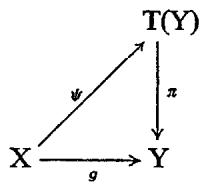
\includegraphics[keepaspectratio]{images/part001_bb2423ff.jpg}}

is commutative, \(\pi\) denoting the canonical projection of T(Y) onto Y. The data of \(\psi\) is equivalent to that of a section of the vector bundle \(g^{*}\mathrm{T}(\mathrm{Y})\), the inverse image under g of T(Y).

The notion of lifting generalizes that of a vector field (to which it reduces when \(g = \operatorname{Id}_{\mathbf{X}}\) ); an important part of the definitions and results concerning \(\theta_{\xi}\) and \(i(\xi)\) extends to liftings; we shall limit ourselves to briefly indicating a few of them.

8.6.2. Let \(\psi: X \to T(Y)\) be a lifting of \(g: X \to Y\) , and let \(\omega\) be a differential form of degree \(p\) on \(Y\) , with values in a vector bundle \(F\) with base \(Y\) . When \(p \geqslant 1\) , one denotes by \(i(\psi,\omega)\) or \(i(\psi)\omega\) or \(i_{\psi}(\omega)\) the differential form on X, of degree \(p-1\) , with values in \(g^{*}\mathbf{F}\) , such that

\[
i (\psi , \omega) _ {x} (v _ {1}, \dots , v _ {p - 1}) = \omega_ {g (x)} (\psi (x), T _ {x} (g). v _ {1}, \dots , T _ {x} (g). v _ {p - 1})\tag{1}
\]

for all \(x \in X\) and every family \(v_1, \ldots, v_{p-1}\) of elements of \(\mathbf{T}_x(X)\) . When \(p = 0\) , we set \(i(\psi, \omega) = 0\) . We say that \(i(\psi, \omega)\) is the interior product of \(\psi\) and of \(\omega\) ; if \(\psi\) and \(\omega\) are of class \(\mathbf{C}^r\) , then so is \(i(\psi, \omega)\) . Let \(\mathbf{F}' \times_{\mathbb{Y}} \mathbf{F}'' \to \mathbf{F}\) be a pairing of vector bundles with base Y. For \(\omega' \in {}^\tau \Omega^{p'}(Y; F')\) and \(\omega'' \in {}^\tau \Omega^{p''}(Y; F'')\) , one has

\[
i (\psi) \left(\omega^ {\prime} \wedge \omega^ {\prime \prime}\right) = (i (\psi) \omega^ {\prime}) \wedge g ^ {*} \omega^ {\prime \prime} + (- 1) ^ {p ^ {\prime}} g ^ {*} \omega^ {\prime} \wedge i (\psi) \omega^ {\prime \prime}.\tag{2}
\]

8.6.3. Examples

\begin{enumerate}
\def\labelenumi{\alph{enumi})}
\tightlist
\item
  A vector field \(\xi\) on X defines a lifting T(g) \(\circ\) \(\xi\) of g in T(Y), and we have:
\end{enumerate}

\[
i (\mathrm{T} (g) \circ \xi) = i (\xi) \circ g ^ {*}.\tag{3}
\]

\begin{enumerate}
\def\labelenumi{\alph{enumi})}
\setcounter{enumi}{1}
\tightlist
\item
  A vector field \(\eta\) on Y defines a lifting \(\eta \circ g\) of \(g\) in T(Y), and we have:
\end{enumerate}

\[
i (\eta \circ g) = g ^ {*} \circ i (\eta).\tag{4}
\]

\begin{enumerate}
\def\labelenumi{\alph{enumi})}
\setcounter{enumi}{2}
\tightlist
\item
  More generally, let \(h: \mathbf{Y} \to \mathbf{Z}\) be a morphism of manifolds of class \(\mathbf{C}^{r+1}\) . If \(\psi\) is a lifting of \(g\) to \(\mathbf{T}(\mathbf{Y})\) , then \(\mathbf{T}(h) \circ \psi\) is a lifting of \(h \circ g\) to \(\mathbf{T}(\mathbf{Z})\) and we have:
\end{enumerate}

\[
i (\mathrm{T} (h) \circ \psi) = i (\psi) \circ h ^ {*}.\tag{5}
\]

If \(\varphi\) is a lifting of \(h\) to \(\mathrm{T}(Z)\) , then \(\varphi \circ g\) is a lifting of \(h \circ g\) to \(\mathrm{T}(Z)\) and we have:

\[
i (\varphi \circ g) = g ^ {*} \circ i (\varphi).\tag{6}
\]

8.6.4 (“Infinitesimal transformations”). Let \(\psi\) be a lifting of class \(C^r\) of \(g\) and let \(\omega\) be a differential form of degree \(p\) on Y, taking values in a Banach space F, and of class \(C^r\) . The differential form on X

\[
d (i (\psi) \omega) + i (\psi) d \omega\tag{7}
\]

is of degree \(p\) and of class \(\mathbf{C}^{r-1}\) ; it is denoted \(\theta_{\psi}.\omega\) .

If f is a function of class \(C^{r}\) on X, we have

\[
\theta_ {f \psi}. \omega = d f \wedge i (\psi) \omega + f \theta_ {\psi}. \omega .\tag{8}
\]

8.6.5 ("Characterization of \(\theta_{\psi}.\omega\) as derivative"). Keep the hypotheses of 8.6.4. Let \(x\in X\) . There then exists an open neighborhood U of \(x\) , an open neighborhood I of 0 in K, and a morphism G: I × U → Y of class \(C^{r}\) having the following two properties:

\begin{enumerate}
\def\labelenumi{\alph{enumi})}
\item
  For every \(x \in \mathbf{U}\) , one has \(\mathbf{G}(0, x) = g(x)\) .
\item
  For every \(x \in \mathbf{U}\) , the image under \(\mathrm{T}_{(0,x)}(\mathrm{G})\) of the tangent vector (1, 0) is equal to \(\psi(x)\) .
\end{enumerate}

Suppose that (U, I, G) satisfies these conditions; for every \(t \in \mathbf{I}\) , denote by \(\mathbf{G}_t\) the map \(x \mapsto \mathbf{G}(t, x)\) from U to Y; set \(\omega_t = \mathbf{G}_t^*(\omega)\) . For every \(x \in \mathbf{X}\) , the map \(t \mapsto \omega_t(x)\) from I to \(\operatorname{Alt}^p(\mathrm{T}_x(\mathbf{X}), \mathbf{F})\) is of class \(\mathbf{C}^r\) , and its derivative at the origin is given by the formula

\[
\frac {d}{d t} (\omega_ {t} (x)) _ {t = 0} = (\theta_ {\psi}. \omega) (x).\tag{9}
\]

\subsection{Weakening of structure}

In this section, we assume K = R.

8.7.1. Let X be a manifold of class \(C^{s}\) , and let F be a vector bundle over X, of class \(C^{k}\) , with \(0 \leqslant k \leqslant s\) . If \(0 \leqslant k' \leqslant k\) , there exists on F a unique structure \(F_{k'}\) of vector bundle with base X and of class \(C^{k'}\) such that every vector chart of F is a vector chart of \(F_{k'}\) . We say that \(F_{k'}\) is obtained from F by weakening the bundle structure of F.

8.7.2. Let \(r \in \mathbf{N}_{\mathbb{R}}\) with \(r \leqslant s\) , and let \(\mathbf{X}_r\) be the manifold of class \(\mathbf{C}^r\) underlying \(\mathbf{X}\) (5.13.1). The tangent bundle \(\mathrm{T}(\mathbf{X}_r)\) is of class \(\mathbf{C}^{r-1}\) ; it is the bundle obtained by weakening of structure from the tangent bundle \(\mathrm{T}(\mathbf{X})\) , which is of class \(\mathbf{C}^{s-1}\) .

Let F be a vector bundle over X, of class \(C^{k}\) , for \(0 \leqslant k \leqslant r - 1\) . The differential forms of class \(C^{k}\) on X with values in F are canonically identified with the corresponding differential forms on \(X_{r}\) . The various operations on these forms described in the rest of this paragraph are compatible with this identification.

In the remainder of this booklet, we will often leave it to the reader to spell out the other results of this kind.

\subsection{Almost complex manifolds and complex manifolds}

In this section, we assume K = R and denote by X a (real) manifold of class \(\mathbf{C}^{r}\) , with \(r \in \mathbf{N}_{\mathbf{R}}\) .

8.8.1 (“Complex vector bundles”). A vector bundle over \(\mathbf{C}\) with base X (7.3.4) is also called a complex vector bundle with base X. If M is such a vector bundle, one calls a complex vector chart of M a triple (U, \(\varphi\) , E), where U is an open subset of X, E a complex Banach space, and \(\varphi\) an isomorphism of complex vector bundles from \(M|_U\) onto the trivial bundle \(E_U = U \times E\). A family \((U_i,\varphi_i,E_i)\) of complex vector charts on M whose domains \(U_i\) cover X is called a complex vector atlas of M; every complex vector bundle possesses a complex vector atlas (7.3.3).

One sometimes says C-vector instead of complex vector. Similarly, when one wishes to speak of a vector bundle over R, of an ordinary vector chart of this bundle, etc., one sometimes says "real vector" or "R-vector" instead of "vector".

Let M be a complex vector bundle with base X. There exists one and only one automorphism j of the (real) vector bundle underlying M (7.3.3) whose restriction to each fibre is multiplication by the element i of C; the square of j is equal to -1. Conversely, if M is a (real) vector bundle with base X and j is an automorphism of M such that \(j^{2} = -1\) , there exists on M a unique structure of complex vector bundle admitting M as underlying (real) vector bundle and for which j is multiplication by i.

8.8.2 ("Complexification of a vector bundle"). One defines a vector functor \(\tau\) by setting \(\tau(E) = E \otimes C\) for every (real) Banach space \(E\) , and \(\tau(u) = u \otimes Id_{C}\) for every morphism \(u: E \to E'\) of (real) Banach spaces.

If F is a vector bundle with base X and of class \(C^{k}\) ( \(0 \leqslant k \leqslant r\) ), its image under the vector functor \(\tau\) is denoted \(F \otimes C\) . There exists on \(F \otimes C\) a unique structure of complex vector bundle with base X and of class \(C^{k}\) , compatible with its structure of (real) vector bundle and inducing on each fibre \((\mathbf{F} \otimes \mathbf{C})_{x} = \mathbf{F}_{x} \otimes \mathbf{C}\) its canonical structure of complex Banach space (EVT, II, § 8, n° 1, Example). Endowed with this structure, one says that \(F \otimes C\) is the complexification of F.

Let U be an open subset of X; the canonical map

\[
\mathcal {S} _ {\mathrm{F}} ^ {k} (\mathrm{U}) \otimes \mathbf {C} \rightarrow \mathcal {S} _ {\mathrm{F} \otimes \mathbf {C}} ^ {k} (\mathrm{U})
\]

is an isomorphism, by which one identifies these two spaces. If \(s \in \mathcal{S}_{\mathrm{F} \otimes \mathrm{C}}^{k}(\mathrm{U})\) , the elements \(\sigma, \tau\) of \(\mathcal{S}_{\mathrm{F}}^{k}(\mathrm{U})\) such that \(s = \sigma + i\tau\) are called the real part and the imaginary part of \(s\) ; the section \(\bar{s} = \sigma - i\tau\) is called the conjugate of \(s\) .

In particular, a section of the bundle \(\mathrm{T}(\mathrm{X}) \otimes \mathbf{C}\) is called a complex vector field on X.

Let H be a complex vector bundle over the base X. The canonical isomorphisms \(\operatorname{Alt}_{\mathbf{R}}^{p}(\mathrm{T}_{x}(\mathrm{X});\mathrm{H})\to\operatorname{Alt}_{\mathbf{C}}^{p}(\mathrm{T}_{x}(\mathrm{X})\otimes\mathbf{C};\mathbf{H})\) define a canonical isomorphism of complex vector bundles, called the canonical one, from \(\operatorname{Alt}_{\mathbf{R}}^{p}(\mathrm{T}(\mathrm{X});\mathrm{H})\) onto \(\operatorname{Alt}_{\mathbf{C}}^{p}(\mathrm{T}(\mathrm{X})\otimes\mathbf{C};\mathbf{H})\) (7.8.5), by means of which we will identify these two bundles. Let \(\omega\) be a section of this bundle, in other words a differential form of degree p on X, with values in H, and let \(\zeta\) be a complex vector field, with real part \(\xi\) and imaginary part \(\eta\). We then set:

\[
i (\zeta , \omega) = i (\xi , \omega) + i. i (\eta , \omega).
\]

If H is a trivial bundle, we set

\[
\theta_ {\zeta}. \omega = \theta_ {\xi}. \omega + i \theta_ {\eta}. \omega .
\]

Similarly, we extend the bracket by linearity to complex vector fields. The formulas of the preceding numbers remain valid.

8.8.3. An almost complex structure of class \(C^{k}\) ( \(k \leqslant r - 1\) ) on X is the data of a complex vector bundle structure on \(\mathrm{T}(\mathrm{X})\), of class \(C^{k}\) , whose underlying real structure is the natural structure of \(\mathrm{T}(\mathrm{X})\). Such a structure is equivalent to the data of an automorphism \(j\) of class \(C^{k}\) of \(\mathrm{T}(\mathrm{X})\) such that \(j^{2} = -1\) .

Let us take such a structure. Extend \(j\) to a \(\mathbf{C}\)-automorphism of \(\mathrm{T}(\mathrm{X}) \otimes \mathbf{C}\). There exists a unique decomposition of \(\mathrm{T}(\mathrm{X}) \otimes \mathbf{C}\) as a direct sum of two complex subbundles:

\[
\mathbf {T} (\mathrm{X}) \otimes \mathbf {C} = \mathbf {T} ^ {\prime} (\mathrm{X}) \oplus \mathbf {T} ^ {\prime \prime} (\mathrm{X})\tag{1}
\]

such that \(j\) coincides with multiplication by \(i\) on \(\mathbf{T}'(\mathbf{X})\) and by \(-i\) on \(\mathbf{T}''(\mathbf{X})\). The projector \(p'\) of \(\mathbf{T}(\mathbf{X}) \otimes \mathbf{C}\) onto \(\mathbf{T}'(\mathbf{X})\) is equal to \(\frac{1}{2}(1 - ij)\) ; the projector \(p'' = 1 - p'\) of \(\mathbf{T}(\mathbf{X}) \otimes \mathbf{C}\) onto \(\mathbf{T}''(\mathbf{X})\) is equal to \(\frac{1}{2}(1 + ij)\) . The composites

\[
\pi^ {\prime} \colon \mathrm{T} (\mathrm{X}) \rightarrow \mathrm{T} (\mathrm{X}) \otimes \mathbf {C} \xrightarrow {p ^ {\prime}} \mathrm{T} ^ {\prime} (\mathrm{X})
\]

\[
\pi^ {\prime \prime}: \mathrm{T} (\mathrm{X}) \rightarrow \mathrm{T} (\mathrm{X}) \otimes \mathbf {C} \xrightarrow {p ^ {\prime \prime}} \mathrm{T} ^ {\prime \prime} (\mathrm{X})
\]

are R-isomorphisms; the first maps j to multiplication by i, the second to multiplication by -i.

8.8.4 (“Forms of type \((p,q)\)"). We keep the hypotheses and notations of the preceding number. Let F be a complex vector bundle with base X, and let p and q be two integers \(\geqslant0\) , and let \(n=p+q\) . Let \(\omega\) be a differential form of degree n on an open set U of X, with values in F; identify (8.8.2) \(\omega\) with a section of \(\operatorname{Alt}_{\mathbf{C}}^{n}(\operatorname{T}(\mathbf{X})\otimes\mathbf{C};\mathbf{F})\) . We say that \(\omega\) is of type \((p,q)\) if, for all \(x\in U\) , one has

\[
\omega_ {x} (v _ {1}, \dots , v _ {n}) = 0
\]

as soon as \(p + 1\) vectors \(v_i\) belong to \(T_x'(X)\) or \(q + 1\) vectors \(v_i\) belong to \(T_x''(X)\). If one identifies \(\bigwedge^n T_x(X) \otimes C\) with the direct sum of the spaces \(\bigwedge^{m'} T_x'(X) \otimes \bigwedge^{m''} T_x''(X)\) for \(m' + m'' = n\) (A, III, p. 85) and \(\omega_x\) with a \(C\)-linear form on \(\bigwedge^n T_x(X)\) , it is equivalent to say that \(\omega_x\) vanishes on \(\bigwedge^{m'} T_x'(X) \otimes \bigwedge^{m''} T_x''(X)\) for \((m', m'') \neq (p, q)\) .

For every pair \((p,q)\) of integers \(\geqslant0\) with \(p+q=n\) there exists a complex vector subbundle \(\operatorname{Alt}^{p,q}(\mathrm{T}(\mathrm{X});\mathrm{F})\) of \(\operatorname{Alt}^{n}(\mathrm{T}(\mathrm{X});\mathrm{F})\) and only one such that its sections over an open set U of X are the differential forms of type \((p,q)\) on X, with values in F. The vector bundle \(\operatorname{Alt}^{n}(\mathrm{T}(\mathrm{X});\mathrm{F})\) is the direct sum of the vector bundles \(\operatorname{Alt}^{p,q}(\mathrm{T}(\mathrm{X});\mathrm{F})\) for \(p\geqslant0\) , \(q\geqslant0\) and \(p+q=n\) . Every differential form \(\omega\) of degree n with values in F decomposes uniquely into

\[
\omega = \sum_ {p + q = n} \omega_ {p, q}
\]

where \(\omega_{p,q}\) is a form of type \((p,q)\) , called the component of type \((p,q)\) of \(\omega\) . If \(\omega\) is of class \(\mathbf{C}^h\) , with \(0 \leqslant h \leqslant k\) , the same holds for its components.

Examples

\begin{enumerate}
\def\labelenumi{\alph{enumi})}
\item
  A differential form of degree n is of type \((n, 0)\) if and only if it is \(\mathbf{C}\)-multilinear.
\item
  Let \(\mathbf{F}'\), \(\mathbf{F}''\), and \(\mathbf{F}\) be three complex vector bundles and let \(\mathbf{F}' \times_{\mathbf{X}} \mathbf{F}'' \to \mathbf{F}\) be a \(\mathbf{C}\)-bilinear pairing. If \(\omega'\) (resp. \(\omega''\)) is a differential form of type \((p',q')\) (resp. \((p'',q'')\)) with values in \(\mathbf{F}'\) (resp. \(\mathbf{F}''\)), the differential form \(\omega' \wedge \omega''\) is of type \((p' + p'',q' + q'')\).
\item
  Suppose that F is the complexification of a (real) vector bundle (8.8.2). If \(\omega\) is a differential form of type \((p, q)\) with values in F, its conjugate \(\overline{\omega}\) (8.8.2) is of type \((q, p)\) .
\end{enumerate}

8.8.5. In addition to the preceding hypotheses, we assume \(k \geqslant 1\) . The following three conditions are then equivalent:

\begin{enumerate}
\def\labelenumi{(\roman{enumi})}
\item
  For every open set U of X and for every pair \((\xi, \eta)\) of complex vector fields on U, of class \(C^{k}\) such that \(\xi(x)\) and \(\eta(x)\) belong to \(\mathrm{T}_{x}^{\prime}(\mathrm{X})\) for all \(x \in U\) , one has \([\xi, \eta](x) \in \mathrm{T}_{x}^{\prime}(\mathrm{X})\) for all \(x \in U\) .
\item
  For every open set U of X and every pair \((\xi, \eta)\) of vector fields (real) on U, of class \(C^{k}\) , one has
\end{enumerate}

\[
[ \xi , \eta ] + j [ j \xi , \eta ] + j [ \xi , j \eta ] - [ j \xi , j \eta ] = 0.
\]

\begin{enumerate}
\def\labelenumi{(\roman{enumi})}
\setcounter{enumi}{2}
\tightlist
\item
  For every open set U of X and for every complex differential form \(\omega\) of type \((1,0)\) on U, of class \(C^{k}\) , the component of type \((0,2)\) of \(d\omega\) is zero.
\end{enumerate}

Suppose these conditions are satisfied. Let \(\omega\) a differential form of type \((p,q)\) on an open set U of X, of class \(\mathbf{C}^h\) with \(1\leqslant h\leqslant k\) with values in a complex Banach space F. We denote by \(d'\omega\) (resp. \(d''\omega\) ) the component of type \((p+1,q)\) (resp. \((p,q+1))\) of \(d\omega\) ; the other components of \(d\omega\) are then zero and one has

\[
d \omega = d ^ {\prime} \omega + d ^ {\prime \prime} \omega .\tag{2}
\]

If \(k\geqslant 2\) , one has

\[
d ^ {\prime} (d ^ {\prime} \omega) = 0, d ^ {\prime \prime} (d ^ {\prime \prime} \omega) = 0, d ^ {\prime} (d ^ {\prime \prime} \omega) + d ^ {\prime \prime} (d ^ {\prime} \omega) = 0.\tag{3}
\]

With the notation of 8.8.4, example \(b\) ), we have

\begin{enumerate}
\def\labelenumi{(\arabic{enumi})}
\setcounter{enumi}{3}
\tightlist
\item
\end{enumerate}

\[
d ^ {\prime} \left(\omega^ {\prime} \wedge \omega^ {\prime \prime}\right) = d ^ {\prime} \left(\omega^ {\prime}\right) \wedge \omega^ {\prime \prime} + (- 1) ^ {p ^ {\prime} + q ^ {\prime}} \omega^ {\prime} \wedge d ^ {\prime} \left(\omega^ {\prime \prime}\right)\tag{4}
\]

\[
d ^ {\prime \prime} (\omega^ {\prime} \wedge \omega^ {\prime \prime}) = d ^ {\prime \prime} (\omega^ {\prime}) \wedge \omega^ {\prime \prime} + (- 1) ^ {p ^ {\prime} + q ^ {\prime}} \omega^ {\prime} \wedge d ^ {\prime \prime} (\omega^ {\prime \prime})\tag{5}
\]

Together with those of 8.8.4, example c), we have

\[
d ^ {\prime} (\overline {{\omega}}) = \overline {{d ^ {\prime \prime} (\omega)}}.\tag{6}
\]

In formulas (4) and (5) (resp. (6)), the differential forms \(\omega'\) and \(\omega''\) (resp. \(\omega\) ) are assumed to be of class \(\mathbf{C}^1\) .

8.8.6 (“Almost complex structure of a complex manifold”). Let \(X^c\) be a complex analytic manifold, admitting X as its underlying real analytic manifold (5.14.2.a)). The bundle \(\mathrm{T}(\mathrm{X})\) is identified with the (real) vector bundle underlying the complex vector bundle \(\mathrm{T}(X^c)\), which endows X with an almost complex structure of class \(C^\omega\) , said to be defined by the given complex analytic manifold structure on X. This almost complex structure satisfies conditions (i) to (iii) of 8.8.5; in particular, the operators \(d'\) and \(d''\) of 8.8.5 are defined. If \(f: X^c \to Y^c\) is a morphism of complex analytic manifolds, \(f^*\) commutes with the operators \(d'\) and \(d''\) .

8.8.7. We retain the hypotheses and notation of 8.8.6. Let \(\overline{\mathbf{X}}^c\) be the conjugate of \(\mathbf{X}^c\) (5.14.2.b)). Embed X by the diagonal map \(x \mapsto (x, x)\) into the complex manifold \(\mathbf{X}^c \times \overline{\mathbf{X}}^c\) , and let \(g\) be the anti-automorphism \((x, y) \mapsto (y, x)\) of \(\mathbf{X}^c \times \overline{\mathbf{X}}^c\) . The pair \((\mathbf{X}^c \times \overline{\mathbf{X}}^c, g)\) is a complexification of X (5.14.8). In particular, for every \(x \in \mathbf{X}\) , the tangent space \(\mathrm{T}_x(\mathrm{X}^c \times \overline{\mathrm{X}}^c)\) is identified with \(\mathrm{T}_x(\mathrm{X}) \otimes \mathbf{C}\) ; in this identification, \(\mathrm{T}_x(\mathrm{X}^c \times \{x\})\) corresponds to \(\mathrm{T}_x'(\mathrm{X})\) and \(\mathrm{T}_x(\{x\} \times \overline{\mathrm{X}}^c)\) corresponds to \(\mathrm{T}_x''(\mathrm{X})\) .

8.8.8. Suppose \(r = \omega\) ; any almost complex structure of class \(C^\omega\) on X satisfying the equivalent conditions (i) to (iii) of 8.8.5 is the almost complex structure defined by one and only one complex analytic manifold structure on \(X\) . \(^{(1)}\)

8.8.9 (“Holomorphic forms”). Let us resume the hypotheses and notations of 8.8.6, and let F be a complex Banach space. The morphic differential forms (in other words, complex analytic ones) on \(\mathbf{X}^c\) with values in F are still called holomorphic differential forms; the identification of \(\mathrm{T}(\mathbf{X}^c)\) with \(\mathrm{T}(\mathbf{X})\) identifies them with (real analytic) differential forms on X. For a differential form \(\omega\) of degree \(p\) on X, with values in F and of class \(\mathbf{C}^k\), with \(k \geqslant 1\), for it to be holomorphic, it is necessary and sufficient that it be of type \((p, 0)\) and that \(d''\omega = 0\) .

Let \(\xi\) be a vector field on X. We say that \(\xi\) is holomorphic if it is a complex analytic mapping from \(X^c\) into \(T(X^c) = T(X)\), in other words, a complex analytic vector field on \(X^c\). If this is the case, and if \(\omega\) is a holomorphic differential form on X with values in F, the form \(\theta_{\xi}.\omega\) (resp. \(i(\xi)\omega\) ) is the same, whether one considers \(\xi\) as a complex analytic vector field on \(X^c\) and \(\omega\) as an element of \(\Omega^p(X^c; F)\) , or \(\xi\) as a vector field on X and \(\omega\) as an element of \(\Omega^p(X; F)\) . Moreover, let \(\xi' = \pi'(\xi)\) and \(\xi'' = \pi''(\xi)\) be the components of \(\xi\) in \(T'(X)\) and \(T''(X)\) respectively (8.8.3); we have

\begin{enumerate}
\def\labelenumi{(\arabic{enumi})}
\setcounter{enumi}{6}
\tightlist
\item
\end{enumerate}
\[
\theta_ {\xi}. \omega = \theta_ {\xi^ {\prime}}. \omega , \quad \theta_ {\xi^ {\prime \prime}}. \omega = 0,\tag{7}
\]

\[
i (\xi) \omega = i (\xi^ {\prime}) \omega , i (\xi^ {\prime \prime}) \omega = 0.\tag{8}
\]

8.8.10. Example. --- Suppose that \(X^{c}\) is an open subset of \(C^{n}\) and denote by \(z^{1},\ldots,z^{n}\) the coordinate functions on \(X^{c}\) . For \(1\leqslant k\leqslant n\) , set \(z^{k}=x^{k}+iy^{k}\) , where \(x^{k}\) and \(y^{k}\) take real values. Consider the tangent frame \((\partial/\partial z^{k})\) of \(\mathrm{T}(\mathrm{X}^{c})\) defined by the coordinate system \((z^{k})\) and the tangent frame \((\partial/\partial x^{k},\partial/\partial y^{k})\) of \(\mathrm{T}(\mathrm{X})\) defined by the coordinate system \((x^{k},y^{k})\) (8.1.5). We have \(j(\partial/\partial x^{k})=\partial/\partial y^{k}\) and the image of \(\partial/\partial z^{k}\) under the map \(\pi^{\prime}\colon\mathrm{T}(\mathrm{X})=\mathrm{T}(\mathrm{X}^{c})\to\mathrm{T}^{\prime}(\mathrm{X})\) (8.8.3) is equal to

\[
\frac {1}{2} (\partial / \partial x ^ {k} - i \partial / \partial y ^ {k});
\]

one generally still denotes it by \(\partial/\partial z^{k}\) . \(^{(2)}\) The complex conjugate vector field of this field \(\partial/\partial z^{k}\) is denoted \(\partial/\partial\bar{z}^{k}\) ; we have

\[
\partial / \partial \bar {z} ^ {k} = \frac {1}{2} (\partial / \partial x ^ {k} + i \partial / \partial y ^ {k}).\tag{9}
\]

If f is a function of class \(C^{1}\) on X, with values in a complex Banach space F, the differential forms \(d'f\) and \(d''f(8.8.5)\) are given by

\[
d ^ {\prime} f = \sum_ {1 \leqslant k \leqslant n} \frac {\partial f}{\partial z ^ {k}} d z ^ {k}, d ^ {\prime \prime} f = \sum_ {1 \leqslant k \leqslant n} \frac {\partial f}{\partial \bar {z} ^ {k}} d \bar {z} ^ {k}.\tag{10}
\]

\(^{(1)}\) If X is of finite dimension, this remains true for an almost complex structure of class \(C^k\) with \(k = \dim X\) (cf. A. Newlander and L. Nirenberg, "Complex analytic coordinates in almost complex manifolds," Ann. of Math. LXX (1957), pp. 391--404).

\(^{(2)}\) Care must be taken: the canonical identification of \(\mathrm{T}(X^c)\) with \(\mathrm{T}(X)\) does not transform the vector field \(\partial/\partial z^k\) on \(X^c\) into the vector field \(\partial/\partial z^k\) on X, but into the vector field \(\partial/\partial z^k+\partial/\partial\bar z^k\). However, the two vector fields denoted \(\partial/\partial z^k\) have the same value on holomorphic differential forms (8.8.9), which are in fact the only forms to which one can apply a vector field of \(X^c\).

Recall that we have

\[
d f = d ^ {\prime} f + d ^ {\prime \prime} f
\]

\[
d z ^ {k} = d x ^ {k} + i d y ^ {k} \quad d \bar {z} ^ {k} = d x ^ {k} - i d y ^ {k}.
\]

If \(\mathbf{A}=(i_{1},\ldots,i_{p})\) is a strictly increasing sequence of integers belonging to the interval \([1,n]\) , we set

\[
d z ^ {A} = d z ^ {i _ {1}} \wedge \dots \wedge d z ^ {i _ {p}}
\]

and denote by \(d\bar{z}^{\mathrm{A}}\) the conjugate of \(dz^{\mathrm{A}}\) . Every differential form \(\omega\) of type \((p,q)\) with values in F is written uniquely as

\[
\omega = \sum_ {\mathrm{A}, \mathrm{B}} f _ {\mathrm{A}, \mathrm{B}} d z ^ {\mathrm{A}} \wedge d \bar {z} ^ {\mathrm{B}}\tag{11}
\]

where A (resp. B) ranges over the set of strictly increasing sequences of \(p\) (resp. \(q\) ) elements of \([1, n]\) , the \(f_{A,B}\) being functions with values in F. If \(\omega\) is of class \(\mathbf{C}^k\) , with \(k \geqslant 1\) , the same holds for the functions \(f_{A,B}\) , and one has

\begin{enumerate}
\def\labelenumi{(\arabic{enumi})}
\setcounter{enumi}{11}
\tightlist
\item
\end{enumerate}
\[
d ^ {\prime} \omega = \sum_ {A, B} d ^ {\prime} f _ {A, B} \wedge d z ^ {A} \wedge d \bar {z} ^ {B}\tag{12}
\]

\[
d ^ {\prime \prime} \omega = \sum_ {\mathbf {A}, \mathbf {B}} d ^ {\prime \prime} f _ {\mathbf {A}, \mathbf {B}} \wedge d z ^ {\mathbf {A}} \wedge d \bar {z} ^ {\mathbf {B}}.\tag{13}
\]

\section{Differential equations and foliations}

In nos. 9.1, 9.2, and 9.3, one assumes that K has characteristic 0. In no. 9.4, one assumes that K has characteristic \(p \neq 0\) .

\subsection{Integral curves}

In this section, X denotes a manifold of class \(C^{r}\) and \(\xi\) is a vector field of class \(C^{s}\) on X, with r, s in \(N_{K}\) , \(s \leqslant r - 1\) .

9.1.1. Let I be an open subset of K, and let \(f: \mathbf{I} \to \mathbf{X}\) a map of class \(\mathbf{C}^k\) ( \(k \in \mathbf{N}_{\mathbb{K}}\) , \(k \leqslant r\) ) from I into X. For \(t \in \mathbf{I}\) , one denotes by \(f'(t)\) the vector \(\mathrm{T}_t(f)(1) \in \mathrm{T}_{f(t)}(\mathbf{X})\) ; this vector is sometimes called the velocity of \(f\) at time \(t\) . When X is a Banach space, \(f'(t)\) is the derivative of \(f\) at \(t\) .

One says that \(f\) is an integral curve of \(\xi\) if one has

\[
f ^ {\prime} (t) = \xi (f (t))\tag{1}
\]

for all \(t \in I\) . Such a curve is of class \(C^{s+1}\) .

If \(x\) is a point of X, one calls integral curve of \(\xi\) with origin \(x\) an integral curve \(f: I \to X\) of \(\xi\) such that \(0 \in I\) and \(f(0) = x\) ; for all \(x \in X\) , there exists an integral curve of \(\xi\) with origin \(x\) , defined in a suitable open neighborhood of 0 in K.

If \(f: \mathbf{I} \to \mathbf{X}\) is an integral curve of \(\xi\) and if \(a \in \mathbf{K}\) , the map \(t \mapsto f(t - a)\) of \(\mathbf{I} + a\) to \(\mathbf{X}\) is an integral curve of \(\xi\) .

Let \(f_{1}\colon\mathbf{I}_{1}\to\mathbf{X}\) and \(f_{2}\colon\mathbf{I}_{2}\to\mathbf{X}\) two integral curves of \(\xi\) , and \(t\in\mathbf{I}_{1}\cap\mathbf{I}_{2}\) . If \(f_{1}(t)=f_{2}(t)\) the maps \(f_{1}\) and \(f_{2}\) coincide in a neighborhood of \(t\) .

9.1.2 ("Flows"). Let W be an open subset of X × K. For every x ∈ X, denote by W \(_{x}\) the set of t ∈ K such that (x, t) ∈ W. We call an integral flow of ξ with domain W a map f of class C \(^{k}\) (k ≤ r) from W to X such that, for every x ∈ X, the map f \(_{x}\) : W \(_{x}\) → X defined by f \(_{x}\) (t) = f(x, t) is an integral curve of ξ, and that whenever (x, 0) ∈ W, one has f(x, 0) = x.

For every point \(x \in X\) , there exists an integral flow of \(\xi\) of class \(\mathbf{C}^s\) whose domain is a neighborhood of \((x, 0)\) in \(X \times K\) . Two integral flows of \(\xi\) defined in a neighborhood of \((x, 0)\) coincide on a neighborhood of \((x, 0)\) .

Let \(x\in X\) and let \(f\) be an integral flow of \(\xi\) whose domain W is a neighborhood of \((x,0)\) . There exists a neighborhood V of \((x,0,0)\) in \(X \times K \times K\) such that, if \((x,t_{1},t_{2})\in\mathrm{V}\) , one has

\[
(x, t _ {1}) \in \mathbf {W}, \quad (f (x, t _ {1}), t _ {2}) \in \mathbf {W}, \quad (x, t _ {1} + t _ {2}) \in \mathbf {W}
\]

and

\[
f (f (x, t _ {1}), t _ {2}) = f (x, t _ {1} + t _ {2}).\tag{2}
\]

If X is paracompact, or if X is separated and K = R or C, there exists an integral flow of \(\xi\) whose domain is a neighborhood of \(X \times \{0\}\) .

9.1.3 ("The real case"). We assume that K = R and that X is separated. We call an integral arc of \(\xi\) any integral curve of \(\xi\) whose domain is an open interval of R. Two integral arcs \(f_{1}\) and \(f_{2}\) of \(\xi\) , defined in intervals \(I_{1}\) and \(I_{2}\) , and coinciding at a point of \(I_{1} \cap I_{2}\) , coincide in \(I_{1} \cap I_{2}\) .

For every point \(x \in X\) , there exists an integral arc with origin \(x\) and one and only one \(f_x: I_x \to X\) such that, for every integral arc \(f: I \to X\) with origin \(x\) , one has \(I \subset I_x\) and \(f = f_x|I\) . The arc \(f_x\) is called the maximal integral arc of \(\xi\) with origin \(x\) , and its domain \(I_x\) is sometimes called the lifetime interval of the point \(x\) for the field \(\xi\) .

If \(I_x = ]-a_-,a_+[\) (and if \(a_+\) is finite, the restriction of \(f_x\) to the interval \([0,a_+[\) is a proper map from \([0,a_+[\) into X. In particular, \(f_x(t)\) has no limit when \(t\) tends to \(a_+\) .

9.1.4. With the notations and hypotheses of 9.1.3, the set \(\Omega\) of the pairs \((x,t)\in\mathbf{X}\times\mathbf{R}\) such that \(t\in\mathbf{I}_{x}\) is open in \(\mathbf{X}\times\mathbf{R}\) and the map \(f\colon\Omega\to\mathbf{X}\) defined by \(f(x,t)=f_{x}(t)\) is an integral flow of \(\xi\) with domain \(\Omega\) .

The functions \(\alpha_{+}\) and \(\alpha_{-}: X \to ]0,+\infty]\) defined by \(I_{x} = ]-\alpha_{-}(x),\alpha_{+}(x)[\) are lower semicontinuous. For \((x, t) \in \Omega\) and \(y = f(x, t)\) , one has \(\alpha_{+}(y) = \alpha_{+}(x) - t\) and \(\alpha_{-}(y) = \alpha_{-}(x) + t\) .

If \(t_1 \in \mathbf{I}_x\) and if \(t_2 \in \mathbf{I}_{f(x, t_1)}\) , one has \(t_1 + t_2 \in \mathbf{I}_x\) and

\[
f (f (x, t _ {1}), t _ {2}) = f (x, t _ {1} + t _ {2}).\tag{3}
\]

If the function \(\alpha_{+}\) (resp. \(\alpha_{-}\) ) is bounded below on X by a constant \(>0\) , it is constant and equal to \(+\infty\) .

One has \(\alpha_{+} = \alpha_{-} = +\infty\) (in other words, one has \(\Omega = \mathbf{X} \times \mathbf{R}\) ) in each of the following cases:

\begin{enumerate}
\def\labelenumi{(\roman{enumi})}
\item
  the field \(\xi\) has compact support (for example if X is compact);
\item
  there exists a transitive group of automorphisms of X preserving \(\xi\) ;
\item
  there exists on X a Riemannian structure for which X is complete and \(\xi\) bounded.
\end{enumerate}

If \(\Omega = X \times R\) , the map \(f: X \times R \to X\) is a right action law of class \(C^s\) of the group manifold \(R\) on the manifold \(X\) , cf.~5.12.5.

9.1.5 ("The complex case"). Suppose that K = C and that X is separated. For every \(a \in ]0, +\infty]\) , denote by \(D_a\) the open disk with center 0 and radius a in C. For every \(x \in X\) , there exists one and only one number \(\rho(x) \in ]0, +\infty]\) and one and only one integral curve \(f_x: D_{\rho(x)} \to X\) with origin \(x\) such that, for every \(a \in ]0, +\infty]\) and every integral curve \(f: \mathrm{D}_a \to \mathrm{X}\) with origin \(x\) , one has \(a \leqslant \rho(x)\) and \(f = f_x | \mathrm{D}_a\) .

For every \(\lambda\in\mathbf{C}\) let \(\alpha_{\lambda}(x)\) be the upper bound of the lifetime interval of \(x\) for the vector field \(\lambda\xi\) on the real manifold deduced from X by restriction of scalars. One has \(\rho(x)=\inf_{|\lambda|=1}\alpha_{\lambda}(x)\) .

The set \(\Delta\) of the pairs \((x,t)\in X\times\mathbf{C}\) such that \(t\in D_{\rho(x)}\) is open in \(X\times\mathbf{C}\) and the map \(f:\Delta\to X\) defined by \(f(x,t)=f_x(t)\) is an integral flow of \(\xi\) . The function \(\rho:X\to ]0,+\infty]\) is lower semicontinuous. For \((x,t)\in\Delta\) and \(y=f(x,t)\) , one has \(\rho(y)\geqslant\rho(x)-|t|\) . If \(\rho\) is bounded below on \(X\) by a constant \(>0\) , one has \(\rho = +\infty\) and \(\Delta = X \times C\) .

When \(\Delta = X \times C\) , the map \(f: X \times C \to X\) is a right action law of the group manifold \(C\) on the manifold \(X\) .

9.1.6. Let \(\varphi: X \to Y\) be a morphism of manifolds and \(\eta\) a vector field on Y such that \(\xi\) is \(\varphi\)-related to \(\eta\) (cf. 8.2.6). If \(f: I \to X\) is an integral curve of \(\xi\) , the map \(\varphi \circ f: I \to Y\) is an integral curve of \(\eta\) . If \(K = R\) and if X and Y are separated, for every \(x \in X\) , the lifetime interval of \(x\) for \(\xi\) is contained in the lifetime interval of \(\varphi(x)\) for \(\eta\) . If moreover \(\varphi\) is proper, these intervals are equal.

9.1.7 ("Time-dependent equations"). Let W be an open subset of X × K and let Ξ: W → T(X) be a lifting of class C \(^{s}\) of pr \(_{1}\) : W → X, that is, a map of class C \(^{s}\) from W into T(X) such that Ξ(x, t) belongs to T \(_{x}\) (X) for all (x, t) ∈ W. One calls an integral curve of Ξ a map f of class C \(^{k}\) (with k ∈ N \(_{K}\) and k ≤ r), from an open subset I of K into X such that, for all t ∈ I, one has

\[
(f (t), t) \in \mathrm{W},\qquad f ^ {\prime} (t) = \Xi (f (t), t).
\]

Let \(\eta\) be the vector field of class \(C^s\) on W defined by \(\eta(x, t) = (\Xi(x, t), (t, 1))\). For a map \(f\) from an open subset I of K into X to be an integral curve of \(\Xi\), it is necessary and sufficient that \(t \mapsto (f(t), t)\) be an integral curve of \(\eta\) in the sense of 9.1.1.

Let \(g: \mathbf{I} \to \mathbf{W}\) be an integral curve of \(\eta\) and \(t_0\) a point of \(\mathbf{I}\) such that \(\operatorname{pr}_2(g(t_0)) = t_0\). The set of elements \(t \in \mathbf{I}\) such that \(\operatorname{pr}_2(g(t)) = t\) is a neighborhood of \(t_0\) that coincides with \(\mathbf{I}\) if \(\mathbf{I}\) is connected.

9.1.8 ("Parameters and initial conditions"). Let Z be a manifold of class \(C^{r}\) , let W be an open subset of X × K × Z , and let \(\Xi\) be a lifting of class \(C^{s}\) of \(pr_{1}: W \to X\). If \(z \in Z\) , one denotes by \(W_{z}\) the set of \((x, t) \in X \times K\) such that \((x, t, z) \in W\) , and one denotes \(\Xi_{z}\) as the map \((x, t) \mapsto \Xi(x, t, z)\) from \(W_{z}\) into T(X).

Let \((x_0, t_0, z_0)\) be a point of W. There then exists an open neighborhood \(X_1 \times I_1 \times Z_1\) of \((x_0, t_0, z_0)\) in W and a map of class \(C^s\)

\[
f \colon X _ {1} \times I _ {1} \times I _ {1} \times Z _ {1} \rightarrow X
\]

such that, for any \((x_{1}, t_{1}, z_{1}) \in \mathbf{X}_{1} \times \mathbf{I}_{1} \times \mathbf{Z}_{1}\) , the map \(t \mapsto f(x_{1}, t_{1}, t, z_{1})\) is an integral curve of \(\Xi_{z_{1}}\) (in the sense of 9.1.7) satisfying the relation \(f(x_{1}, t_{1}, t_{1}, z_{1}) = x_{1}\) .

Two maps

\[
f _ {1}: \mathrm{X} _ {1} \times \mathrm{I} _ {1} \times \mathrm{I} _ {1} \times \mathrm{Z} _ {1} \rightarrow \mathrm{X} \quad \text {and} \quad f _ {2}: \mathrm{X} _ {2} \times \mathrm{I} _ {2} \times \mathrm{I} _ {2} \times \mathrm{Z} _ {2} \rightarrow \mathrm{X}
\]

satisfying the above conditions coincide in a neighborhood of \((x_{0}, t_{0}, t_{0}, z_{0})\) .

\subsection{Foliations}

In this section, X denotes a manifold of class C \(^{r}\) , with \(r \in \mathrm{N}_{\mathrm{K}}\) . Unless otherwise stated, all manifolds and morphisms considered are assumed to be of class C \(^{r}\) .

9.2.1. Let S be a manifold, and let \(p: X \to S\) be a submersion. For every \(s \in S\) , we endow \(X_s = p^{-1}(s)\) with the manifold structure induced by that of X (5.10.5); the set X is the disjoint union of the \(X_s\) . Denote by \(X_p\) the manifold structure on X obtained by gluing the \(X_s\) , for \(s \in S\) (5.2.4); it is the unique manifold structure on X for which the \(X_s\) are open submanifolds. The topological space \(X_p\) is the sum of the spaces \(X_s\) .

Let V be a manifold and \(f\) a map from V into X. For \(f\) to be a morphism from V to \(\mathbf{X}_{p}\), it is necessary and sufficient that \(f\) be a morphism from V to X and that \(p \circ f\) be locally constant.

9.2.2. A foliation of X is a manifold Y having the same underlying set as X and satisfying the following condition:

\begin{enumerate}
\def\labelenumi{(\Alph{enumi})}
\setcounter{enumi}{5}
\tightlist
\item
  For every \(x \in X\) , there exists an open submanifold U of X containing x, a manifold S, and a submersion \(p: U \to S\) such that the manifold \(U_{p}\) is an open submanifold of Y.
\end{enumerate}

We also say that the pair (X, Y) is a foliated manifold. If (X, Y) and (X', Y') are foliated manifolds, a morphism from (X, Y) to (X', Y') is any map \(f: X \to X'\) which is both a morphism from the manifold X to the manifold X' and a morphism from the manifold Y to the manifold Y'.

Let (X, Y) be a foliated manifold. The identity map Y → X is a bijective immersion. A subset U of X is called a leaf if it is an open set of Y; in this case, U is endowed with the topological structure and the manifold structure induced by those of Y; for example, U is said to be a connected leaf if it is an open and connected subset of Y. The leaves that are submanifolds of X form a basis for the topology of Y. When K = R or C, the connected components of Y are leaves, called the maximal connected leaves of (X, Y).

9.2.3. If \(s \in \mathbf{N}_{\mathbb{K}}\) , \(s \leqslant r\) , we call a foliation of class \(\mathbf{C}^s\) of \(\mathbf{X}\) a foliation of the manifold of class \(\mathbf{C}^s\) underlying \(\mathbf{X}\) .

9.2.4. Examples

\begin{enumerate}
\def\labelenumi{\alph{enumi})}
\item
  The manifold X is a foliation of X, called the coarse foliation of X.
\item
  If \(p: \mathbf{X} \to \mathbf{S}\) is a submersion, \(\mathbf{X}_p\) is a foliation of \(\mathbf{X}\) called the foliation of \(\mathbf{X}\) defined by \(p\) . The foliation of \(\mathbf{X}\) defined by the identity map is the set \(\mathbf{X}\) endowed with its structure of a pure manifold of dimension 0 (5.2.1); it is called the discrete foliation of \(\mathbf{X}\) .
\item
  Let E be a Banach space, F a closed vector subspace of E admitting a topological complement, and p the canonical projection \(E \rightarrow E/F\) . The foliation \(E_{p}\) of E is called the foliation of E defined by F.
\item
  Let \(\Gamma\) be a discrete group acting properly and freely on the topological space X (TG, III, § 4, no. 4). Let Y be a foliation of X, and suppose that, for every \(s \in \Gamma\) , the map \(x \mapsto sx\) is an automorphism of (X, Y). The equivalence relation on X (resp. Y) whose classes are the orbits of \(\Gamma\) is regular (5.9.5). If we denote by X/\(\Gamma\) (resp. Y/\(\Gamma\)) the corresponding quotient manifold, the pair (X/\(\Gamma\),Y/\(\Gamma\)) is a foliated manifold, called the quotient of (X, Y) by \(\Gamma\) .
\end{enumerate}

9.2.5. Let Y be a foliation of X and U an open subset of X. Then U is open in Y, and U, endowed with the manifold structure induced by that of Y, is a foliation of X, called the foliation induced by Y.

More generally, let \(f: X' \to X\) be a morphism such that \(f\) and the identity map \(Y \to X\) form a transversal pair (5.11.1). The fibered product \(Y' = X' \times_X Y\) is canonically identified with a foliation of \(X'\) called the pullback foliation of \(Y\) by \(f\) .

9.2.6. Let \(p: \mathbf{X} \to \mathbf{S}\) and \(p': \mathbf{X}' \to \mathbf{S}'\) be two submersions, and let \(f\) be a morphism from \(\mathbf{X}\) to \(\mathbf{X}'\) . For \(f\) to be a morphism from \(\mathbf{X}_p\) to \(\mathbf{X}_{p'}\) , it is necessary and sufficient that, for every \(x \in \mathbf{X}\) , there exists an open neighborhood \(\mathbf{U}\) of \(x\) in \(\mathbf{X}\) and a morphism \(g\) from \(p(\mathbf{U})\) to \(\mathbf{S}'\) such that \(g \circ p = p' \circ f\) on \(\mathbf{U}\) .

9.2.7. Let Y be a foliation of X. A foliated chart of (X, Y) is a quadruple (U, \(\varphi\) , E, F) such that (U, \(\varphi\) , E) is a chart of X, F is a closed vector subspace of the Banach space E admitting a topological complement, and \(\varphi\) is an isomorphism from the foliation of U induced by Y to the foliation of \(\varphi(\mathbf{U})\) defined by the canonical mapping from E onto E/F. For every point \(x \in \mathbf{X}\) there exists a foliated chart (U, \(\varphi\), E, F) of (X, Y) such that \(x \in \mathbf{U}\) . Let \(n = \dim_x \mathbf{X}\) and let \(m = \dim_x \mathbf{Y}\) . If \(n\) is finite, there exists an open neighborhood U of \(x\) and a coordinate system \(\zeta^1, \ldots, \zeta^n\) of X over U such that the foliation of U induced by Y coincides with the foliation defined by the map (\(\zeta^{m+1}, \ldots, \zeta^n\)) from U into \(\mathbf{K}^{n-m}\) .

9.2.8. Let Y be a foliation of X. When x ranges over X, the spaces \(T_{x}(Y)\) are the fibers of a vector subbundle of class \(C^{r-1}\) of T(X), which is called the subbundle of T(X) tangent to the foliation Y and is denoted T(X, Y). If the foliation Y is defined by a submersion \(p: X \to S\) , then T(X, Y) = Ker T(p) is the relative tangent bundle T(X/S) of X over S (8.1.3).

Let (X, Y) and (X', Y') be two foliated manifolds, and let f be a morphism from X to X'. For f to be a morphism of foliated manifolds, it is necessary and sufficient that T(f) map T(X, Y) into T(X', Y'). In particular, let \(f: Z \to X\) be a morphism of manifolds; for f to be a morphism from Z to Y, it is necessary and sufficient that T(f) map T(Z) into T(X, Y). For a submanifold Z of X to be a leaf of (X, Y), it is necessary and sufficient that one have

\[
\mathrm{T} _ {z} (\mathrm{Z}) = \mathrm{T} _ {z} (\mathrm{X}, \mathrm{Y}) \quad \text {for all} \quad z \in \mathrm{Z}.
\]

Let Y be a foliation of X and let U be a leaf of Y, admitting a countable base of open sets. Let Z be a manifold and f a map from Z to U. For f to be a morphism of manifolds from Z to U, it is necessary and sufficient that the composite of f and the canonical injection of U into X be a morphism of manifolds from Z to X. If X is locally compact and countable at infinity, every connected leaf of (X, Y) admits a countable base of open sets (cf.~TG, I, 3rd ed., §11, no. 7, cor. 2 of th. 1).

9.2.9. Suppose that K = R or C. Let Y be a foliation of X. The following conditions are equivalent:

\begin{enumerate}
\def\labelenumi{\alph{enumi})}
\item
  There exist a manifold S and a submersion \(p: X \to S\) such that \(Y = X_p\) .
\item
  For every \(x \in X\) , there exists a submanifold \(S_{x}\) of X possessing the following two properties:
\begin{enumerate}
\item[\(b_1)\)] The tangent space \(\mathbf{T}_{x}(\mathbf{S}_{x})\) to \(\mathbf{S}_{x}\) at \(x\) is a topological supplement of \(\mathbf{T}_{x}(\mathbf{X},\mathbf{Y})\) in \(\mathbf{T}_{x}(\mathbf{X})\) .
\item[\(b_2)\)] Every connected leaf of (X, Y) intersects \(S_{x}\) at at most one point.
\end{enumerate}
\end{enumerate}

Suppose these conditions are satisfied, and let R be the relation on X “x and y belong to the same connected leaf”; then R is a regular equivalence relation (5.9.5) on X, and, if p denotes the canonical projection \(X \to X/R\), we have \(Y = X_p\) .

Example. --- Take K = R and X = R². Let the discrete group Γ = Z² act on X by translations. Let m ∈ R and let (X, Yₘ) be the foliation defined by the submersion p: (x₁, x₂) ↦ x₂ - mx₁ from X onto R. Set X' = X/Γ and Yₘ' = Yₘ/Γ; then Yₘ' is a foliation of the torus X' (cf.~9.2.4, example d)). If m is rational, there exists a submersion p' from X' onto R/Z such that Yₘ' = Xₚ'. If m is irrational, every maximal connected leaf of (X', Yₘ') is dense in X', and there does not exist a submersion p' from X' into a manifold S such that Yₘ' = Xₚ'.

9.2.10. Let Y be a foliation of X, and let \(\pi: X \to S\) be a morphism of manifolds such that the composite \(Y \to X \xrightarrow{\pi} S\) is étale. If \(S'\) is an open subset of S, a section \(\sigma: S' \to X\) of \(\pi\) above \(S'\) is said to be horizontal (with respect to the foliation Y) if it is a morphism from \(S'\) into Y; it is equivalent to say that \(\sigma(S')\) is a leaf of (X, Y), or again that \(T(\sigma)\) maps \(T(S')\) to \(T(X, Y)\) . For every \(s_0 \in S\) and for every \(x_0 \in \pi^{-1}(s_0)\) , there exists a horizontal section defined in a neighborhood of \(s_0\) and taking the value \(x_0\) at \(s_0\) ; two such sections coincide on a neighborhood of \(s_0\) .

More generally, let \(s_{0}\in S\) , let T be a manifold, let \(f\) be a morphism from T into the submanifold \(\pi^{-1}(s_{0})\) of X, and let \(t_{0}\in T\) . There then exists an open neighborhood \(\mathbf{T}^{\prime}\) (resp. \(S'\)) of \(t_{0}\) in T (resp. of \(s_{0}\) in S), and a morphism

\[
\mathbf {F}: \mathbf {S} ^ {\prime} \times \mathbf {T} ^ {\prime} \rightarrow \mathbf {X}
\]

satisfying the following condition: for every \(t \in \mathbf{T}'\) , the map \(s \mapsto \mathrm{F}(s, t)\) is a horizontal section of \(\pi\) above \(\mathbf{S}'\) taking the value \(f(t)\) at the point \(s_0\) . Two such maps F coincide on a neighborhood of \((s_0, t_0)\) .

\subsection{Integrable subbundles}

In this section, X denotes a manifold of class \(C^{r}\) and F a vector subbundle of class \(C^{s}\) of T(X), with r, s in \(N_{K}\) , \(s \leqslant r - 1\) .

9.3.1. Let V be a manifold of class \(C^{k}\) ( \(k \in N_{K}, k \leqslant r\) ) and let f be a morphism of class \(C^{k}\) from V into X. We say that f is an integral of F if T(f) maps T(V) into F.

A submanifold Z of class \(C^{k}\) of X is called an integral submanifold of F if the injection \(Z \rightarrow X\) is an integral of F in the above sense, i.e. if one has \(\mathrm{T}_{x}(\mathbf{Z}) \subset \mathrm{F}_{x}\) for all \(x \in Z\) .

Let \(x \in X\) . If \(Z_1\) and \(Z_2\) are two integral submanifolds of \(F\) containing \(x\) and if \(T_x(Z_1) = F_x\) , there exists a neighborhood \(U\) of \(x\) such that \(U \cap Z_2 \subset Z_1\) . If moreover \(T_x(Z_2) = F_x\) , the germs of \(Z_1\) and \(Z_2\) at \(x\) coincide.

9.3.2. We say that F is integrable if there exists a foliation Y of X of class \(C^{s}\) such that \(F = T(X, Y)\) (9.2.8). Such a foliation is then unique; it is called the integral foliation of F. For a morphism f: \(V \to X\) of class \(C^{s}\) to be an integral of F, it is necessary and sufficient that f be a morphism from V into Y.

Example. --- If F has rank 1 at every point, F is integrable, and defines on X a pure foliation of dimension 1. Suppose moreover that K = R, that X is separated, and that F admits as a frame a vector field \(\xi\) nowhere zero. Then, for every \(x \in X\) , the maximal connected leaf containing \(x\) is the image of the maximal integral arc of \(\xi\) with origin \(x\) (9.1.3).

9.3.3 ("Integrability criteria"). The following conditions are equivalent:

\begin{enumerate}
\def\labelenumi{(\roman{enumi})}
\item
  The vector subbundle F of T(X) is integrable.
\item
  For every \(x \in X\) , there exists an integral submanifold \(Z\) of class \(C^s\) of \(F\) such that \(x \in Z\) and \(T_x(Z) = F_x\) .
\item
  For every open set U of X and vector fields \(\xi\) and \(\eta\) belonging to \(\mathcal{S}_{\mathbf{F}}^{s}(\mathbf{U})\) (7.4.1), one has \([\xi, \eta] \in \mathcal{S}_{\mathbf{F}}^{s-1}(\mathbf{U})\) .
\end{enumerate}

Let \((\xi_{i})_{i\in I}\) be a family of sections of F of class \(C^{s}\) such that, for every \(x\in X\) , the set of the \(\xi_{i}(x)\) is a total subset of the Banach space \(F_{x}\) (EVT, I, § 2, no. 1). The conditions (i), (ii), and (iii) are then equivalent to:

\begin{enumerate}
\def\labelenumi{(\roman{enumi})}
\setcounter{enumi}{3}
\tightlist
\item
  for every pair \((i,j)\) of elements of I and every \(x\in X\) , one has \([\xi_i,\xi_j](x)\in F_x\) .
\end{enumerate}

When I is finite and the family \((\xi_{i})\) is a frame of F, the preceding conditions are still equivalent to:

\begin{enumerate}
\def\labelenumi{(\alph{enumi})}
\setcounter{enumi}{21}
\tightlist
\item
  there exists a family \((c_{ij}^{k})_{(i,j,k)\in I\times I\times I}\) of functions on \(X\) with values in \(K\) such that \([\xi_i,\xi_j] = \sum_{k}c_{ij}^k\xi_k\) for all \(i,j\) in \(I\) .
\end{enumerate}

(If this is the case, the functions \(c_{i,j}^{k}\) are of class \(\mathbf{C}^{s-1}\) .)

9.3.4. Let \(s' \in \mathbf{N}_{\mathbb{K}}\) , with \(s' \leqslant s\) , and let \(\mathbf{F}'\) be the vector bundle of class \(\mathbf{C}^{s}\) deduced from \(\mathbf{F}\) by weakening of structure (8.7.1). For \(\mathbf{F}\) to be integrable, it is necessary and sufficient that \(\mathbf{F}'\) be integrable. In this case, the integral foliation of \(\mathbf{F}'\) is deduced from that of \(\mathbf{F}\) by weakening of structure.

9.3.5. Let E be a Banach space and \(p\) be an integer \(\geqslant 0\) . For every \(x \in X\) , denote by

\(N(p, E)_{x}\) the vector subspace of \(\text{Alt}^{p}(T_{x}(X); E)\) consisting of the elements \(u\) such that \(u(v_{1}, \ldots, v_{p}) = 0\) for \(v_{1}, \ldots, v_{p}\) in \(F_{x}\) . The spaces \(N(p, E)_{x}\) , for \(x \in X\) , are the fibers of a vector subbundle of class \(C^{s}\) of \(\text{Alt}^{p}(T(X); E)\) . Denote it by \(N(p, E)\) . If \(F\) is integrable, we have:

\begin{enumerate}
\def\labelenumi{(\roman{enumi})}
\setcounter{enumi}{5}
\tightlist
\item
  for every open set U of X and every form \(\omega \in \mathcal{S}_{\mathrm{N}(p,\mathbb{E})}^s (\mathrm{U})\) , one has \(d\omega \in \mathcal{S}_{\mathrm{N}(p + 1,\mathbb{E})}^{s - 1}(\mathrm{U})\) .
\end{enumerate}

Conversely, if (vi) holds for \(p=1\) and for every Banach space E, the bundle F is integrable; when K = R or C, it even suffices to verify (vi) for \(p=1\) and E = K.

Suppose that the dual of T(X)/F admits a frame \((\omega_{1},\ldots,\omega_{n})\) . The integrability of F is then equivalent to the following condition:

\begin{enumerate}
\def\labelenumi{(\roman{enumi})}
\setcounter{enumi}{6}
\tightlist
\item
  \[
  d \omega_ {i} \wedge \omega_ {1} \wedge \dots \wedge \omega_ {n} = 0 \quad \text {for} \quad 1 \leqslant i \leqslant n.
  \]
\end{enumerate}

If moreover there exists a vector subbundle G of class \(C^{s}\) of T(X) such that T(X) is the direct sum of F and G, condition (vii) is equivalent to:

\begin{enumerate}
\def\labelenumi{(\roman{enumi})}
\setcounter{enumi}{7}
\tightlist
\item
  there exist differential forms \(\alpha_{i}^{j}\) ( \(i, j\) in I) of degree 1 on X, of class \(\mathbf{C}^{s-1}\) , such that \(d\omega_{i} = \sum_{j} \alpha_{i}^{j} \wedge \omega_{j}\) for all \(i \in \mathbf{I}\) .
\end{enumerate}

9.3.6. Let L be a Banach space and let \(\omega\) be a differential form of degree 1 on X with values in L, of class C \(^{s}\) . We make the following two hypotheses:

\begin{enumerate}
\def\labelenumi{\alph{enumi})}
\item
  for all \(x \in \mathbf{X}\) , \(\omega_x\) is a surjective homomorphism of \(\mathrm{T}_x(\mathbf{X})\) to \(\mathbf{L}\) , and the kernel of \(\omega_x\) is \(\mathrm{F}_x\) ;
\item
  there exists a vector subbundle G of T(X) such that T(X) is the direct sum of F and G.
\end{enumerate}

The integrability of F is then equivalent to:

\begin{enumerate}
\def\labelenumi{(\roman{enumi})}
\setcounter{enumi}{8}
\tightlist
\item
  there exists a differential form \(\alpha\) of degree 1 on X with values in \(\operatorname{End}(\mathbf{L})\) such that \(d\omega = \alpha \wedge \omega\) , the exterior product being defined by the canonical pairing \(\operatorname{End}(\mathbf{L}) \times \mathbf{L} \to \mathbf{L}\) (7.8.2 and 8.3.2).
\end{enumerate}

9.3.7 ("Equations in total differentials"). Suppose that X is the product of two manifolds A and B of class \(C^{r}\) ; one denotes \(p_{1}: X \to A\) and \(p_{2}: X \to B\) the two projections. Let f be a morphism of class \(C^{s}\) of \(p_{1}^{*}T(A)\) to \(p_{2}^{*}T(B)\) . The graphs of the maps \(f_{(a,b)}: T_{a}(A) \to T_{b}(B)\) are the fibers of a vector subbundle of class \(C^{s}\) of \(T(X)\) ; denote it by \(F^{f}\) .

Let A' be an open subset of A, and let \(\varphi: \mathbf{A}' \to \mathbf{B}\) be a morphism of class \(\mathbf{C}^k\) ( \(k \in \mathbb{N}_{\mathbb{K}}\) , \(k \leqslant r\) ). One says that \(\varphi\) is an integral of \(f\) if, for all \(a \in \mathbf{A}'\) , one has \(\mathrm{T}_a(\varphi) = f_{a,\varphi(a)}\) ; this is equivalent to saying that the map \(a \mapsto (a, \varphi(a))\) of \(\mathbf{A}'\) into X is an integral of \(\mathbf{F}^f\) (9.3.1). Such a map is of class \(\mathbf{C}^{s+1}\) . If \(\varphi_1\) and \(\varphi_2\) are two integrals of \(f\) and take the same value at a point \(a \in \mathbf{A}\) , they coincide in a neighborhood of \(a\) .

More generally, let Z be a manifold of class \(C^{k}\) , let A' be an open subset of A, let \(a \in A'\) and let \(\Phi_{1}, \Phi_{2}\) be morphisms of class \(C^{k}\) from \(Z \times A'\) into B.

\(\Phi_{1}\) and \(\Phi_{2}\) coincide on \(Z \times \{a\}\) and that, for all \(z \in Z\) , the morphisms

\[
a \mapsto \Phi_ {1} (z, a) \quad \text {and} \quad a \mapsto \Phi_ {2} (z, a)
\]

are integrals of \(f\) . Then \(\Phi_{1}\) and \(\Phi_{2}\) coincide in a neighborhood of \(Z \times \{a\}\) .

Suppose that \(F^{f}\) is integrable. Let Z be a manifold of class \(C^{k}\) ( \(k \in \mathbf{N}_{\mathbb{K}}, k \leqslant s\) ), \((z_{0}, a_{0})\) a point of \(Z \times A\) , and \(\rho\) be a morphism of class \(C^{k}\) from Z into B. There exists an open neighborhood \(Z' \times A'\) of \((z_{0}, a_{0})\) in \(Z \times A\) and a morphism \(\Phi: Z' \times A' \to B\) of class \(C^{k}\) such that, for all \(z \in Z'\) , the map \(a \mapsto \Phi(z, a)\) from \(A'\) into B admits f as its tangent map and takes the value \(\rho(z)\) at the point \(a_{0}\) .

9.3.8. We retain the hypotheses and notation of 9.3.7 and suppose that A (resp. B) is an open submanifold of a Banach space E (resp. M). The map f then identifies with a morphism of class C \(^{s}\) from X = A × B into the Banach space \(\mathcal{L}(E; M)\) . Let D \(_{1}\) f (resp. D \(_{2}\) f) denote the first (resp. second) partial derivative of f (1.6.2); it is a morphism of class C \(^{s-1}\) from X into \(\mathcal{L}(E; \mathcal{L}(E; M))\) (resp. into \(\mathcal{L}(M; \mathcal{L}(E; M))\) ), a space identified in the obvious way with \(\mathcal{L}_{2}(E; M)\) (respectively with \(\mathcal{L}(M, E; M)\) ). For F to be integrable, it is necessary and sufficient that, for every x ∈ X, the bilinear map

\[
\Delta_ {x}: (h _ {1}, h _ {2}) \mapsto \mathrm{D} _ {1} f (x) (h _ {1}, h _ {2}) + \mathrm{D} _ {2} f (x) (f (x) h _ {1}, h _ {2})
\]

from \(E \times E\) to M be symmetric. Under this condition, if \(\varphi\) is an integral of f defined in an open subset A' of A, the second derivative of \(\varphi\) at a point \(a\) of A' is \(\Delta(a,\varphi(a))\).

If \(E = K^n\) , and if one denotes \((x^1, \ldots, x^n)\) the coordinate functions on \(K^n\) , the map \(f\) is defined by a family \((f_1, \ldots, f_n)\) of maps from \(A \times B\) to \(M\) , and the integrability condition is written:

\[
\frac {\partial f _ {i}}{\partial x ^ {j}} + (\mathbf {D} _ {2} f _ {i}). f _ {j} = \frac {\partial f _ {j}}{\partial x ^ {i}} + (\mathbf {D} _ {2} f _ {j}). f _ {i}
\]

for all integers \(i, j\) in \([1, n]\) . A map \(\varphi\) of an open subset A' of A into B is an integral of \(f\) if and only if one has

\[
\frac {\partial \varphi}{\partial x ^ {i}} = f _ {i} (x, \varphi (x)) \quad \text {for all} \quad x \in \mathbf {A} ^ {\prime} \text { and all } i \in [ 1, n ],
\]

in other words, if one has

\[
d \varphi = \sum_ {1 \leqslant i \leqslant n} f _ {i} (x, \varphi (x)) d x ^ {i}.
\]

\subsection{\texorpdfstring{Integrable bundles in characteristic \(p \neq 0\)}{Integrable bundles in characteristic p nonzero}}

In this number, we assume K has characteristic \(p \neq 0\) . We denote by X a K-analytic manifold locally of finite dimension.

9.4.1 ("p-th powers"). Let \(\xi\) be a vector field on an open subset U of X. There exists a vector field \(\xi^p\) and only one on U such that we have

\[
\mathrm{D} _ {\xi^ {p}} (f) = (\mathrm{D} _ {\xi}) ^ {p} (f) = \underbrace {\mathrm{D} _ {\xi} (\mathrm{D} _ {\xi} (\dots (\mathrm{D} _ {\xi} (f)) . . .))} _ {p \text { times }}\tag{1}
\]

for every analytic function f defined in an open subset of U.

If \(\varphi\) is an analytic function on U, we have

\[
(\varphi \xi) ^ {p} = \varphi^ {p} \xi^ {p} + (\mathrm{D} _ {\varphi \xi}) ^ {p - 1} (\varphi). \xi\tag{2}
\]

and if \(\eta\) is a vector field on U, we have

\[
[ \xi^ {p}, \eta ] = \operatorname{ad}(\xi) ^ {p} (\eta) = [ \xi , [ \xi , \dots , [ \xi , \eta ] \dots ] ].\tag{3}
\]

9.4.2 ("Jacobson's identity"). Let L be the free \(F_{p}\)-Lie algebra (LIE, II, § 2, no. 2) on a set \(\{x, y\}\) with two elements. There exists one and only one element \(\Lambda_{p}(x, y)\) of L such that we have

\[
(x + y) ^ {p} = x ^ {p} + y ^ {p} + \Lambda_ {p} (x, y)\tag{4}
\]

in the enveloping algebra of L. Examples:

\[
\Lambda_ {2} (x, y) = [ x, y ]; \quad \Lambda_ {3} (x, y) = [ x, [ x, y ] ] - [ y, [ x, y ] ].
\]

If \(\xi\) and \(\eta\) are vector fields on X, we have

\[
(\xi + \eta) ^ {p} = \xi^ {p} + \eta^ {p} + \Lambda_ {p} (\xi , \eta).\tag{5}
\]

9.4.3. Example. --- Take \(X = K\) (resp. \(K^*\)) and denote by x the canonical map \(X \to K\). Let \(\xi\) (resp. \(\eta\)) be the vector field \(\partial/\partial x\) (resp. \(x\cdot\partial/\partial x\)); it is invariant under translations of the additive (resp. multiplicative) group X. We have

\[
\xi^ {p} = 0 \quad \text { and } \quad \eta^ {p} = \eta .\tag{6}
\]

9.4.4 (“Integrable bundles”). Let F be a vector subbundle of T(X). We say that F is integrable if, for every \(x \in X\) , there exists a coordinate system (\(\zeta^{1}, \ldots, \zeta^{n}\)) of X at x and an integer \(m \leqslant n\) such that \((\partial/\partial\zeta^{1}, \ldots, \partial/\partial\zeta^{m})\) is a frame of F in a neighborhood of x.

For F to be integrable, it is necessary and sufficient that it satisfy the following condition:

For every open set U of X, \(\mathcal{S}_{\mathbb{F}}^{\omega}(\mathbf{U})\) is a Lie subalgebra of \(\mathcal{S}_{\mathrm{T}(\mathbf{X})}^{\omega}(\mathbf{U})\) stable under the operation \(\xi \mapsto \xi^{p}\) .

\section{Measures defined by differential forms}

In this paragraph, we assume that K is locally compact. From Section 10.2 onward, we assume K = R. In Sections 10.1 and 10.4, all manifolds considered are assumed to be locally of finite dimension; when they are Hausdorff, they are locally compact.

\subsection{Modulus measure of a differential form}

Notation. --- We denote \(\mu\) a Haar measure (INT, VII, §1, no. 2) on the additive group of K. We denote \(\mu^{\otimes n}\) the measure \(\mu \otimes \cdots \otimes \mu\) onto \(K^n\) and \(\mu_{\mathbf{U}}^{\otimes n}\) its restriction to an open set U of \(K^n\) . For \(a \in K\) we denote by mod(a) the modulus of a (INT, VII, §1, no. 10 and AC, VI, §9, no. 1). If K = R, we have mod(a) = \textbar a\textbar; if K = C, we have mod(a) = \textbar a\textbar\^{}2; if K is ultrametric, we have mod(a) = \(q^{-v(a)}\) , where \(q\) denotes the number of elements in the residue field of K \(v\) the normalized valuation of K (AC, VI, §9, no. 1, prop. 1).

10.1.1. Let U and V be open subsets of \(K^{n}\) and let f: \(U \to V\) a map of class \(C^{r}\) , with \(r \in N_{K}\) . Let \(x \in U\) ; we call the Jacobian of f at x, and denote by \(\operatorname{Jac}_{x}(f)\) , the determinant of the linear map \(Df(x)\) derivative of f at x. We denote \(\operatorname{Jac}(f)\) the function \(x \mapsto \operatorname{Jac}_{x}(f)\) the function \(\operatorname{mod}(\operatorname{Jac}(f))\) is a continuous function in U with positive real values.

10.1.2 ("Change of variable in integrals"). Under the hypotheses of 10.1.1, suppose that \(f\) let be a class isomorphism \(\mathbf{C}^{r}\) of the manifold U onto the manifold V. Then the image under \(f\) of the measure mod(Jac(f)). \(\mu_{\mathrm{U}}^{\otimes n}\) is \(\mu_{\mathrm{V}}^{\otimes n}\) ; for every continuous function with compact support \(\varphi: \mathrm{V} \to \mathbf{C}\) , one has

\[
\int_ {\mathrm{V}} \varphi (y) \mu^ {\otimes n} (y) = \int_ {\mathrm{U}} \varphi (f (x)). \mathrm{mod} (\operatorname{Jac} _ {x} (f)) \mu^ {\otimes n} (x).\tag{1}
\]

10.1.3. Let X be a variety of class \(\mathbf{C}^r\) and let A be a subset of X. One says that A is locally negligible if, for every chart \((\mathrm{U},\varphi ,\mathrm{K}^n)\) of the manifold X, the set \(\varphi (\mathrm{A}\cap \mathrm{U})\) is \(\mu^{\otimes n}\)-negligible (INT, IV, § 2, no. 2); this condition does not depend on the choice of \(\mu\) , and it suffices to verify it for a family of charts whose domains cover A. Every set contained in the union of a countable family of locally negligible sets is locally negligible.

Examples

\begin{enumerate}
\def\labelenumi{\alph{enumi})}
\item
  Every submanifold of X that has codimension \(\geqslant1\) at every point (i.e. has empty interior) is locally negligible.
\item
  Let g be a function of class \(C^{r}\) on X, and let \(A_{g}\) the set of points \(x \in X\) such that \(g(x) = 0\) ; suppose that the interior of \(A_{g}\) is empty, and that \(r = \omega\) ; then \(A_{g}\) is locally negligible.
\item
  Let \(f: Y \to X\) be a morphism of manifolds of class \(C^{r}\) , the manifold \(Y\) being a countable union of compact sets. It is assumed that one has \(\dim_{y} Y \leqslant \dim_{f(y)} X\) for all \(y \in Y\) . Its image under \(f\) of every locally negligible subset of \(Y\) is a locally negligible subset of \(X\) . The same is true of the image under \(f\) of the set of points where \(f\) is not étale (“first Sard theorem”); in particular, if \(\dim_{y} Y < \dim_{f(y)} X\) for all \(y \in Y\) , \(f(Y)\) is a locally negligible subset of \(X\) .
\item
  Suppose K has characteristic zero. Let \(f\colon Y\to X\) be a morphism of manifolds of class \(\mathbf{C}^{r}\) ( \(r\in N_{K}, r\geqslant\infty\) ), Y being a countable union of compact sets. Let C be the set of points of Y where \(f\) is not a submersion (“critical points”). Then \(f(\mathbf{C})\) is a locally negligible subset of X (“second Sard theorem”). \(^{(1)}\)
\end{enumerate}

10.1.4. Let X be a paracompact manifold of class C'. On X there exists a class M of equivalent measures (INT, V, § 5, n° 6), and only one, such that, for every \(\nu \in \mathbf{M}\) and for every chart \(c = (\mathrm{U}, \varphi, \mathrm{K}^n)\) of X, the image under \(\varphi\) of the restriction of \(\nu\) to U is equivalent to \(\mu_{\varphi(\mathrm{U})}^{\otimes n}\) . One says that M is the canonical class of measures on X. For a subset A of X to be locally negligible (10.1.3), it is necessary and sufficient that it be locally negligible (INT, IV, § 2, n° 2) for one (resp. every) measure \(\nu \in \mathbf{M}\) .

If K = R and \(r \neq \omega\) (resp. K = R or C and \(r = \omega\) , resp. K is ultrametric), there exists \(\nu \in M\) such that, for every chart \(c = (\mathrm{U}, \varphi, \mathrm{K}^{n})\) of X, the density of \(\varphi(\nu_{\mathrm{U}})\) with respect to \(\mu_{\varphi(\mathrm{U})}^{\otimes n}\) is everywhere \textgreater0 and of class \(C^{r-1}\) (resp. of class \(C^{\infty}\) , resp. locally constant). If \(\nu\) and \(\nu'\) are two such measures, the density of \(\nu'\) with respect to \(\nu\) is everywhere \textgreater0 and of class \(C^{r-1}\) (resp. of class \(C^{\infty}\) , resp. locally constant).

10.1.5. Let X be a manifold of class \(\mathbf{C}^r\) ; let \(\mathrm{T}'(\mathrm{X})\) the cotangent bundle of X (8.2.2) and set \(\Omega = \det(\mathrm{T}'(\mathrm{X}))\) (7.9.9). The vector bundle \(\Omega\) has rank 1 at each point; when X is pure of dimension \(n\) , it is identified with the vector bundle \(\operatorname{Alt}^n(\mathrm{T}(\mathrm{X}); \mathrm{K}_{\mathbf{x}})\) . Let \(\omega\) a section of \(\Omega\) on X; one says, by abuse of language, that \(\omega\) is a differential form of maximum degree on X. Let \(c = (\mathrm{U}, \varphi, \mathrm{K}^n)\) be a chart of X; denote by \(u^1, \ldots, u^n\) the coordinate functions on \(\mathrm{K}^n\) . There exists a function \(f_c\) and only one on \(\varphi(\mathrm{U})\) such that \(\omega|_{\mathrm{U}} = \varphi^*(f_c.du^1 \wedge \cdots \wedge du^n)\) . We say that \(\omega\) is locally of integrable modulus if, for every chart \(c = (\mathrm{U}, \varphi, \mathrm{K}^n)\) of X, the real function mod \((f_c)\) : \(\varphi(\mathrm{U}) \to \mathbf{R}\) is locally integrable for \(\mu_{\varphi(\mathrm{U})}^{\otimes n}\) (INT, IV, § 4, n° 1); it suffices to verify this property for the charts of an atlas of X. If \(\omega\) is continuous, and in particular if \(\omega\) is of class \(\mathbf{C}^s\), with \(s \in \mathbb{N}_{\mathbf{K}}, s \leqslant r - 1\), then \(\omega\) is locally of integrable modulus.

10.1.6 (“Positive measure defined by a differential form of maximum degree”). Keep the notations of 10.1.5 and suppose moreover that X is separated and that \(\omega\) is locally of integrable modulus. If \(c = (\mathrm{U}, \varphi, \mathrm{K}^n)\) is a chart of X, denote by \(\nu_c\) the measure on \(\varphi(\mathrm{U})\) product of the measure \(\mu_{\varphi(\mathrm{U})}^{\otimes n}\) by the function mod( \(f_c\) ) (INT, V, § 5, n° 2, def. 2) and let \(\alpha_c\) the image of \(\nu_c\) by \(\varphi^{-1}\) . There exists on X a measure \(\alpha\) and only one such that, for every chart \(c = (\mathrm{U}, \varphi, \mathrm{K}^n)\) of X, the restriction of \(\alpha\) to U is equal to \(\alpha_c\) . One says that the measure \(\alpha\) is the modulus of \(\omega\) and one denotes it mod( \(\omega\) ) \(_\mu\) . It is a positive measure. When K = R and \(\mu\) is Lebesgue measure, one writes \(|\omega|\) instead of mod( \(\omega\) ) \(_\mu\) .

If X is purely of dimension n, and if a is a real number \textgreater0, one has \(\text{mod}(\omega)_{a\mu} = a^{n} \text{ mod}(\omega)_{\mu}\) .

Let A be a subset of X. For A to be locally negligible (10.1.3), it is necessary and sufficient that, for every open set U of X and every differential form \(\omega\) of maximum degree on U which is locally of integrable modulus, the set A ∩ U be locally negligible for the measure mod( \(\omega\) ) \(_{\mu}\) .

Suppose moreover X is paracompact and let \(\nu\) be a measure on X belonging to the canonical equivalence class M (10.1.4). The measure mod \((\omega)_{\mu}\) is based on \(\nu\) (INT, V, § 5, no. 2, def. 2). For mod \((\omega)_{\mu}\) to belong to M, it is necessary and sufficient that the set of \(x \in \mathbf{X}\) such that \(\omega(x) = 0\) be locally negligible.

10.1.7. Example. --- Let G be a Lie group over K, of finite dimension n, and let \(\omega\) be a differential form of degree n on G, invariant under left translations, and nonzero. The corresponding measure \(\text{mod}(\omega)_{\mu}\) is then a left Haar measure on the locally compact group G.

When G is the multiplicative group \(K^{*}\) , one may take for \(\omega\) the form dx/x, and one has \(\text{mod}(\omega)_{\mu} = (\text{mod})^{-1}.\mu\) , cf.~INT, VII, § 1, no. 10, prop. 14.
\begin{enumerate}
\def\labelenumi{(\arabic{enumi})}
\setcounter{enumi}{6}
\tightlist
\item
\end{enumerate}
